% =============================================================================
% Punto 5 — Mapas de correlación con el clima global
% Cuenca Río Maipo en El Manzano (CAMELS-CL 5710001)
% Figuras y tablas: scripts/15_p5_1 (descarga), 16_p5_1, 17_p5_2, 18_p5_3, 19_p5_4
% Compilar desde documentos/:  pdflatex punto5_teleconexiones_analisis.tex
% Las líneas "% VERIFICAR" señalan datos o referencias por contrastar con la fuente.
% =============================================================================
\documentclass[11pt,letterpaper]{article}
\usepackage[utf8]{inputenc}
\usepackage[T1]{fontenc}
\usepackage[spanish,es-nodecimaldot,es-noshorthands]{babel}
\usepackage{lmodern}
\usepackage[margin=2.3cm]{geometry}
\usepackage{amsmath,amssymb}
\usepackage{graphicx}
\usepackage{booktabs}
\usepackage{tabularx}
\usepackage{float}
\usepackage{caption}
\usepackage{xcolor}
\usepackage{tcolorbox}
\usepackage[numbers,sort&compress]{natbib}
\usepackage[hidelinks]{hyperref}
\graphicspath{{../figuras/}}
\captionsetup{font=small,labelfont=bf}

\title{Punto 5. Mapas de correlación con el clima global\\
\large Río Maipo en El Manzano (CAMELS-CL 5710001)}
\author{Tarea 1 de Hidrología, UNAL Medellín}
\date{}

\begin{document}
\sloppy
\maketitle

\noindent\textbf{Pregunta.} ¿Qué regiones oceánicas y patrones atmosféricos se asocian con la variabilidad mensual
de la precipitación y el caudal de la cuenca, y cómo cambia esa asociación según el mes del año?

\section{Campos climáticos seleccionados (5.1)}

Se usaron tres campos mensuales globales del reanálisis ERA5 \citep{Hersbach2020}, descargados del Copernicus
Climate Data Store con \texttt{scripts/15\_p5\_1\_descargar\_campos\_era5.py} (Tabla~\ref{tab:campos}). La
elección responde a la cadena física que lleva la lluvia invernal a Chile central:
\begin{itemize}
\item \textbf{SST}: es el forzante de las teleconexiones tropicales. ENSO modula la frecuencia de los
sistemas frontales y de los bloqueos que alcanzan Chile central \citep{Rutllant1991,Montecinos2003}.
\item \textbf{Presión al nivel del mar (PNM)}: describe la intensidad y la posición del anticiclón subtropical
del Pacífico Sur, que bloquea o deja pasar los frentes. La lluvia de la cuenca depende de que ese
anticiclón se debilite o se desplace \citep{Garreaud2009}.
\item \textbf{Altura geopotencial en 500 hPa (Z500)}: identifica vaguadas y bajas segregadas en la tropósfera
media, que pueden producir precipitación aun sin un frente en superficie, y completa la PNM en la vertical.
\end{itemize}
Se distingue el geopotencial $\Phi$ (m$^2$\,s$^{-2}$, la variable de ERA5) de la altura geopotencial
$Z=\Phi/g_0$ (m, $g_0=9.80665$~m\,s$^{-2}$), que es la que se analiza. Al ser un nivel de presión alto, a
500~hPa no hay celdas bajo la superficie.

\begin{table}[H]
\centering\footnotesize
\caption{Campos climáticos utilizados (\texttt{figuras/tabla\_5\_1\_metadatos\_campos.csv}).}
\label{tab:campos}
\begin{tabularx}{\textwidth}{l X l l X}
\toprule
Campo & Producto CDS (DOI) & Unidades & Rango verificado & Máscara \\
\midrule
SST & ERA5 \emph{single levels monthly means} (10.24381/cds.f17050d7), \texttt{sea\_surface\_temperature} & K $\rightarrow$ $^\circ$C & $-1.6$ a 36.3 $^\circ$C & Tierra y hielo marino (SST $\leq-1.6$~$^\circ$C, el punto de congelación que ERA5 asigna bajo hielo) \\
PNM & ídem, \texttt{mean\_sea\_level\_pressure} & Pa $\rightarrow$ hPa & 958.8 a 1048.5 hPa & Ninguna \\
Z500 & ERA5 \emph{pressure levels monthly means} (10.24381/cds.6860a573), \texttt{geopotential}, 500 hPa & m$^2$\,s$^{-2}$ $\rightarrow$ m & 4655 a 5969 m & Ninguna \\
\bottomrule
\end{tabularx}
\end{table}
% VERIFICAR el DOI del producto de niveles de presión en la página de CDS.

Para los tres campos: tipo \emph{monthly averaged reanalysis}, enero de 1979 a diciembre de 2020 (504 meses, sin
faltantes), dominio global y malla regular de 1$^\circ$. La resolución nativa es 0.25$^\circ$; la malla de
1$^\circ$ la interpoló CDS en la descarga y es adecuada para patrones de gran escala. Se incluyó 1979 para
poder usar rezagos (enero de 1980 con $\ell=1$ se empareja con diciembre de 1979). Del lado de la cuenca, la
precipitación de referencia $P_L$ y el caudal $Q$ aportan 38--41 años por mes calendario (1980--2020). IMERG
($P_I$) y la temperatura aportan solo 19--20, así que IMERG se usa únicamente como contraste
(Sección~\ref{sec:robustez}). La Figura~\ref{fig:clim} muestra la climatología invernal y la variabilidad
interanual de cada campo: la variabilidad de la SST es máxima en el Pacífico ecuatorial oriental (ENSO), y la
de la PNM y la Z500 en las latitudes altas del Pacífico sur.

\begin{figure}[H]
\centering
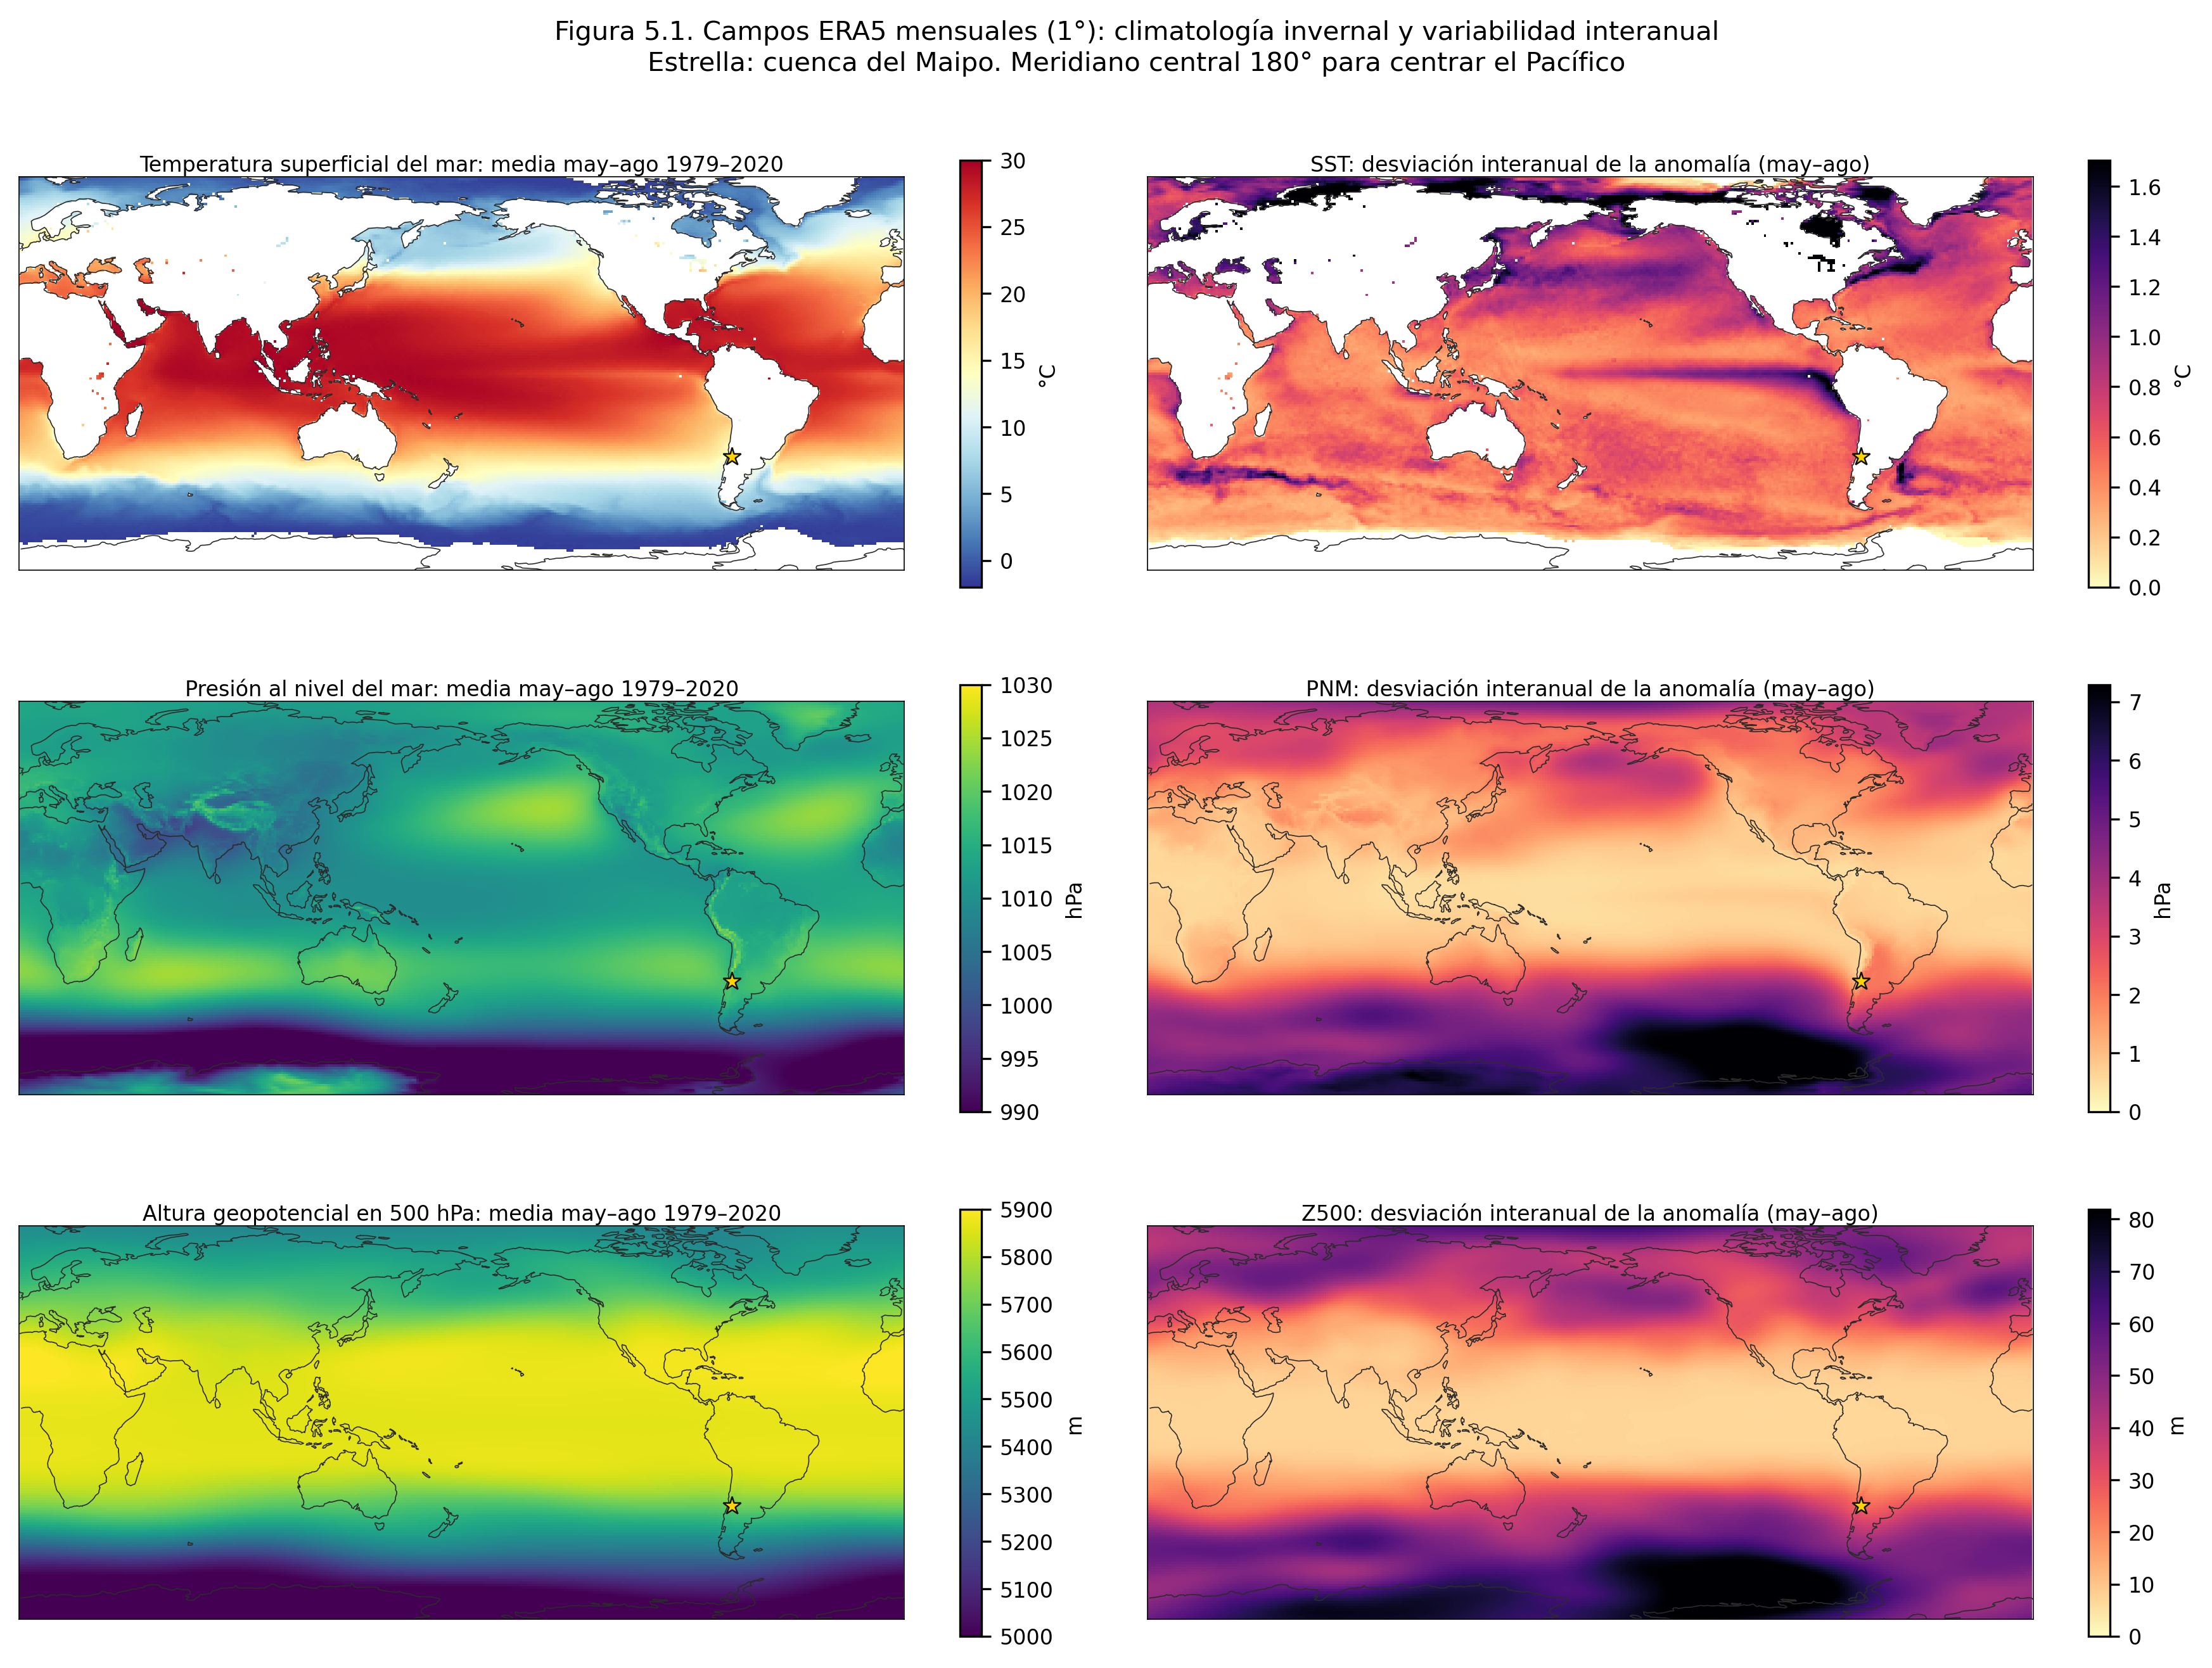
\includegraphics[width=\textwidth]{figura_5_1_climatologia_campos.png}
\caption{Climatología de mayo a agosto (izquierda) y desviación estándar interanual de la anomalía (derecha) de
la SST, la PNM y la Z500. Estrella: cuenca. Script \texttt{16\_p5\_1\_campos\_climaticos.py}.}
\label{fig:clim}
\end{figure}

\section{Definición y cálculo de los mapas (5.2)}

Para cada mes calendario $j$ de la respuesta de la cuenca y cada celda $(\lambda,\phi)$:
\begin{equation}
r_j(\lambda,\phi;\ell)=\operatorname{corr}_{\{t:\,j(t)=j\}}\big[a_X(t),\,a_Y(\lambda,\phi,t-\ell)\big],
\end{equation}
donde $a_X$ y $a_Y$ son anomalías por mes calendario respecto de la referencia fija 2000-06 a 2020-03, la
misma usada para la cuenca en los puntos 1 a 4. La correlación se calcula \emph{a través de los años}: por
ejemplo, todos los julios de $P_L$ con todos los julios de la PNM en esa celda. Para un mes fijo, centrar las
series no cambia Pearson, por lo que los mapas de valores originales y de anomalías son idénticos y se muestra
una sola versión. El mapa base es sin rezago ($\ell=0$). Además se evaluó un rezago justificado
físicamente: $Q$ frente a la SST seis meses antes, porque el caudal de deshielo depende de la nieve acumulada en
el invierno anterior (desfase de 6--7 meses de los puntos 1 y 2). Con la convención $\ell>0$ el campo antecede a
la cuenca.

Las Figuras~\ref{fig:pl_sst}--\ref{fig:q_z500} presentan los 12 mapas de cada combinación. Los mapas de
$P_L$ y $Q$ frente a la Z500 y a la PNM de $Q$ se incluyen por completitud; los resultados centrales se
resumen en las secciones siguientes.

\begin{figure}[H]
\centering
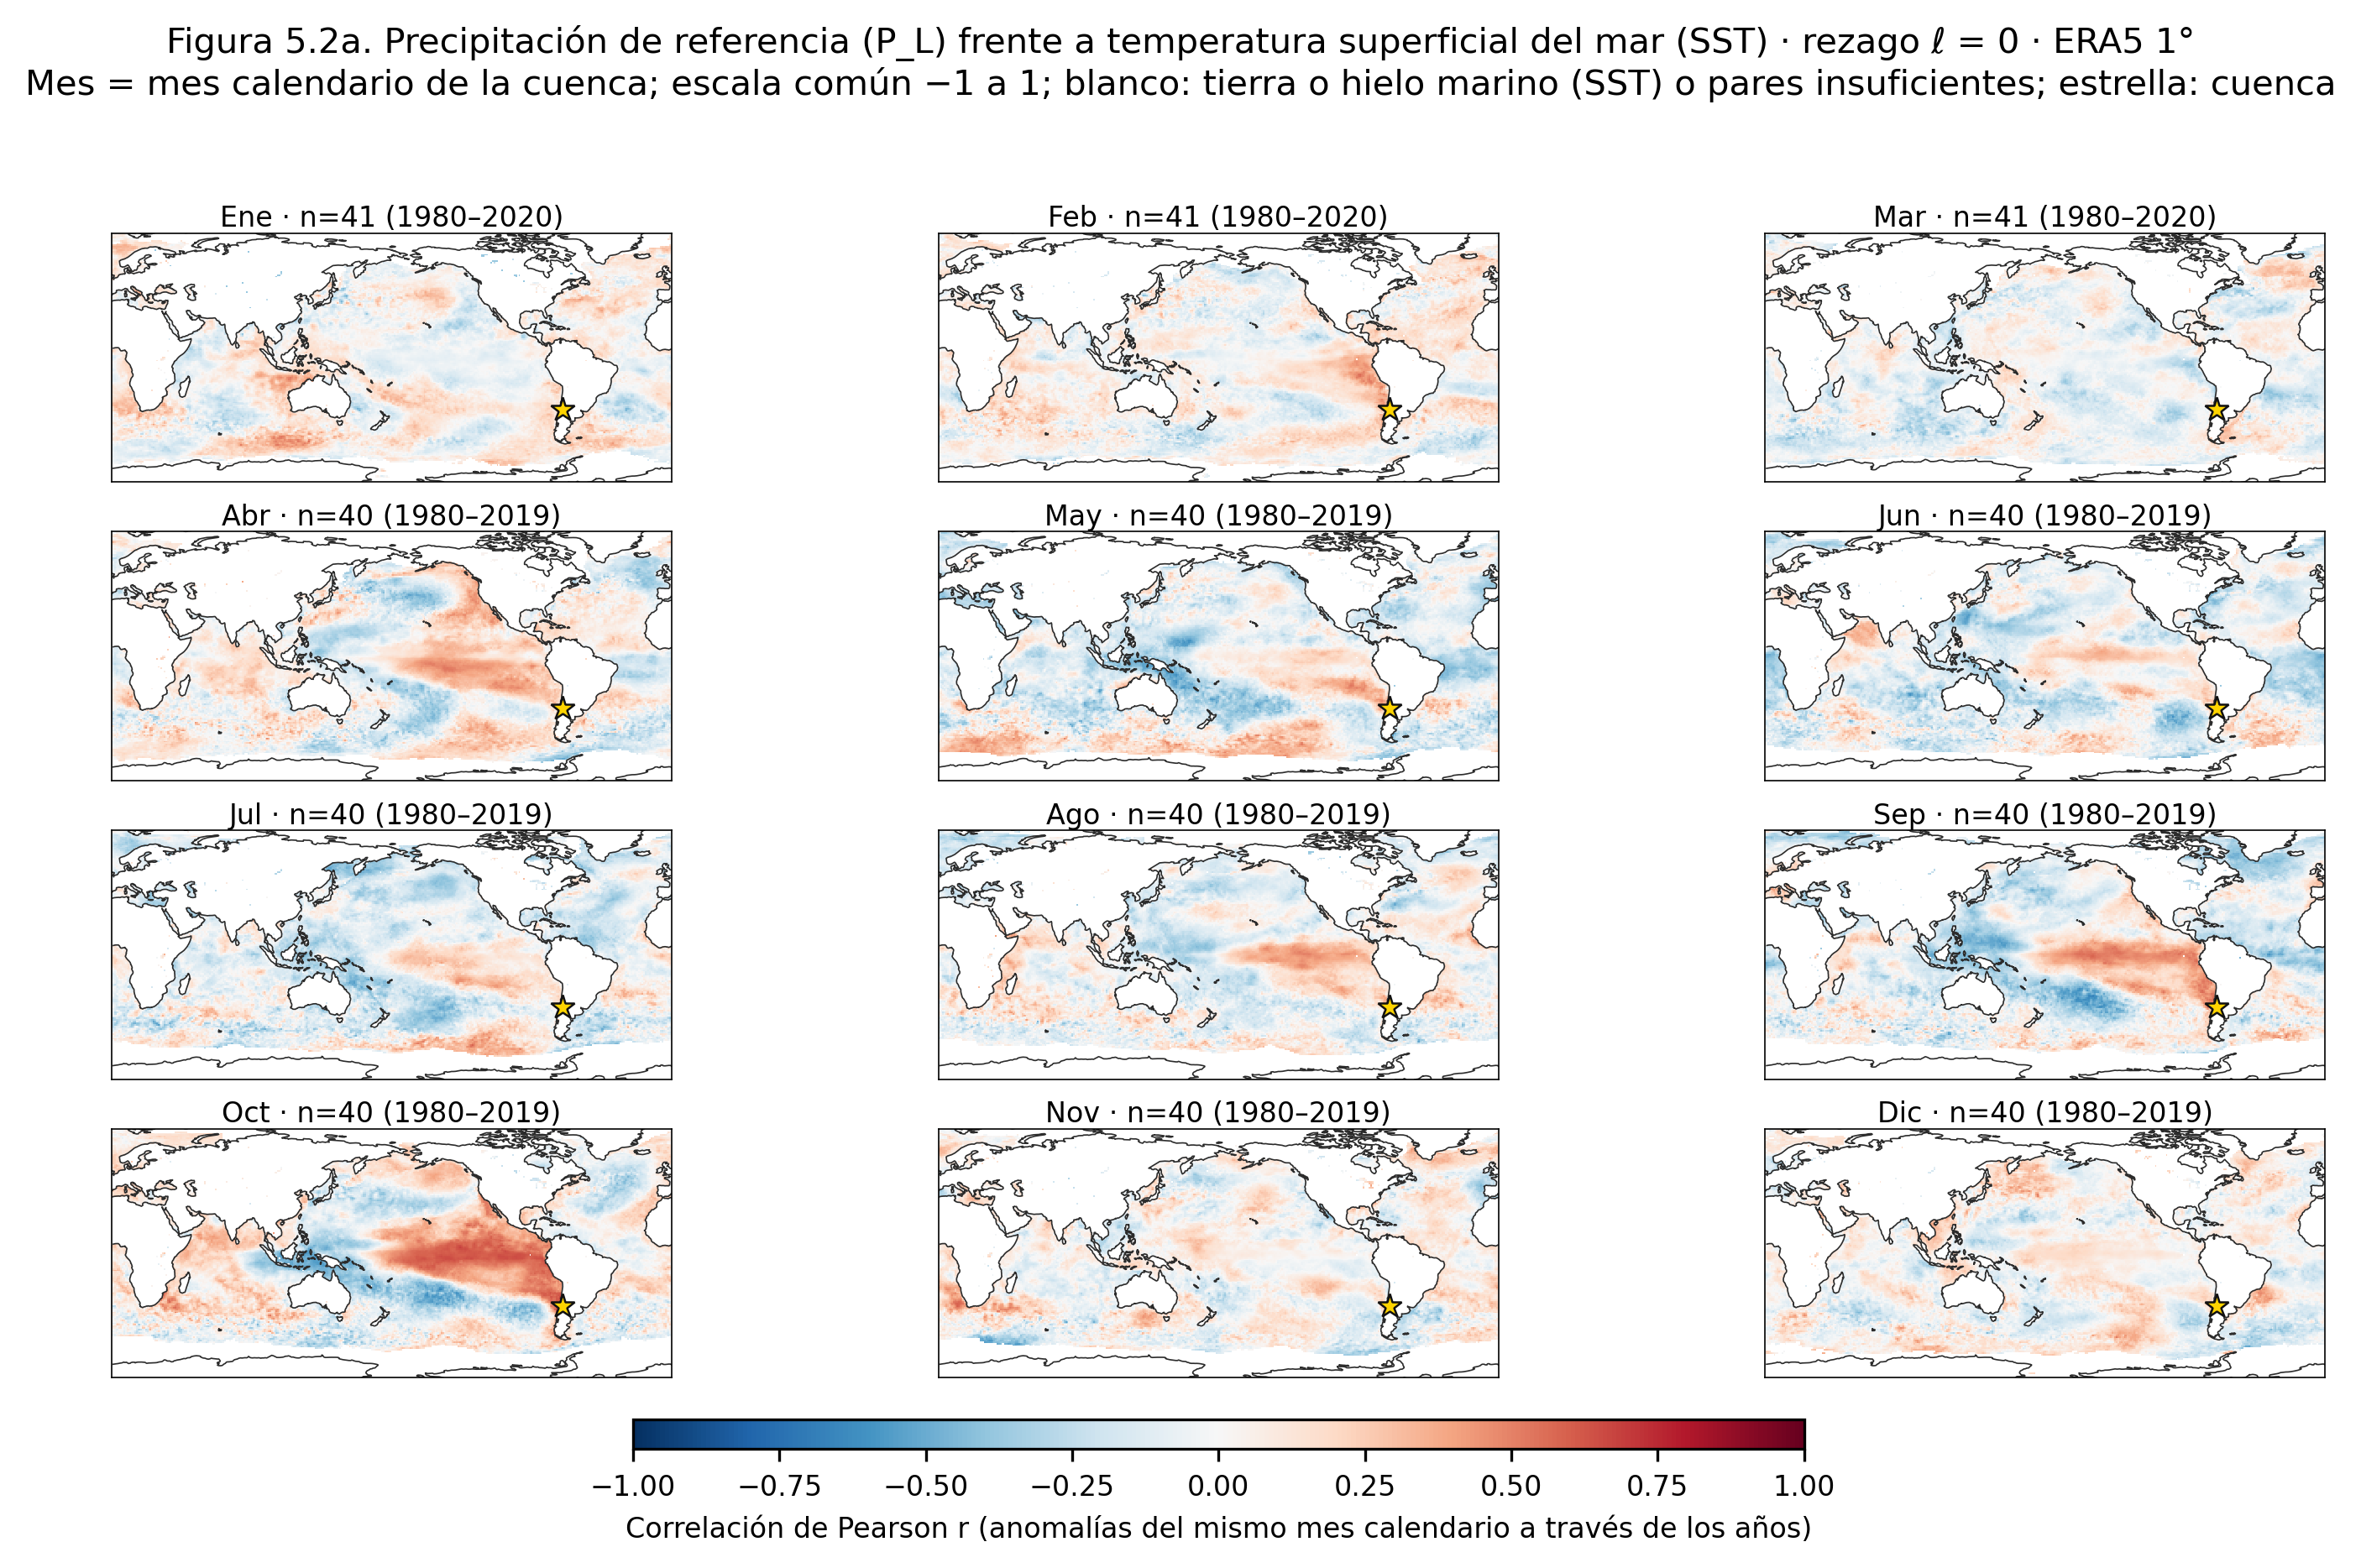
\includegraphics[width=\textwidth]{figura_5_2a_p_l_sst.png}
\caption{$P_L$ frente a SST, $\ell=0$. Script \texttt{17\_p5\_2\_mapas\_correlacion.py}.}
\label{fig:pl_sst}
\end{figure}

\begin{figure}[H]
\centering
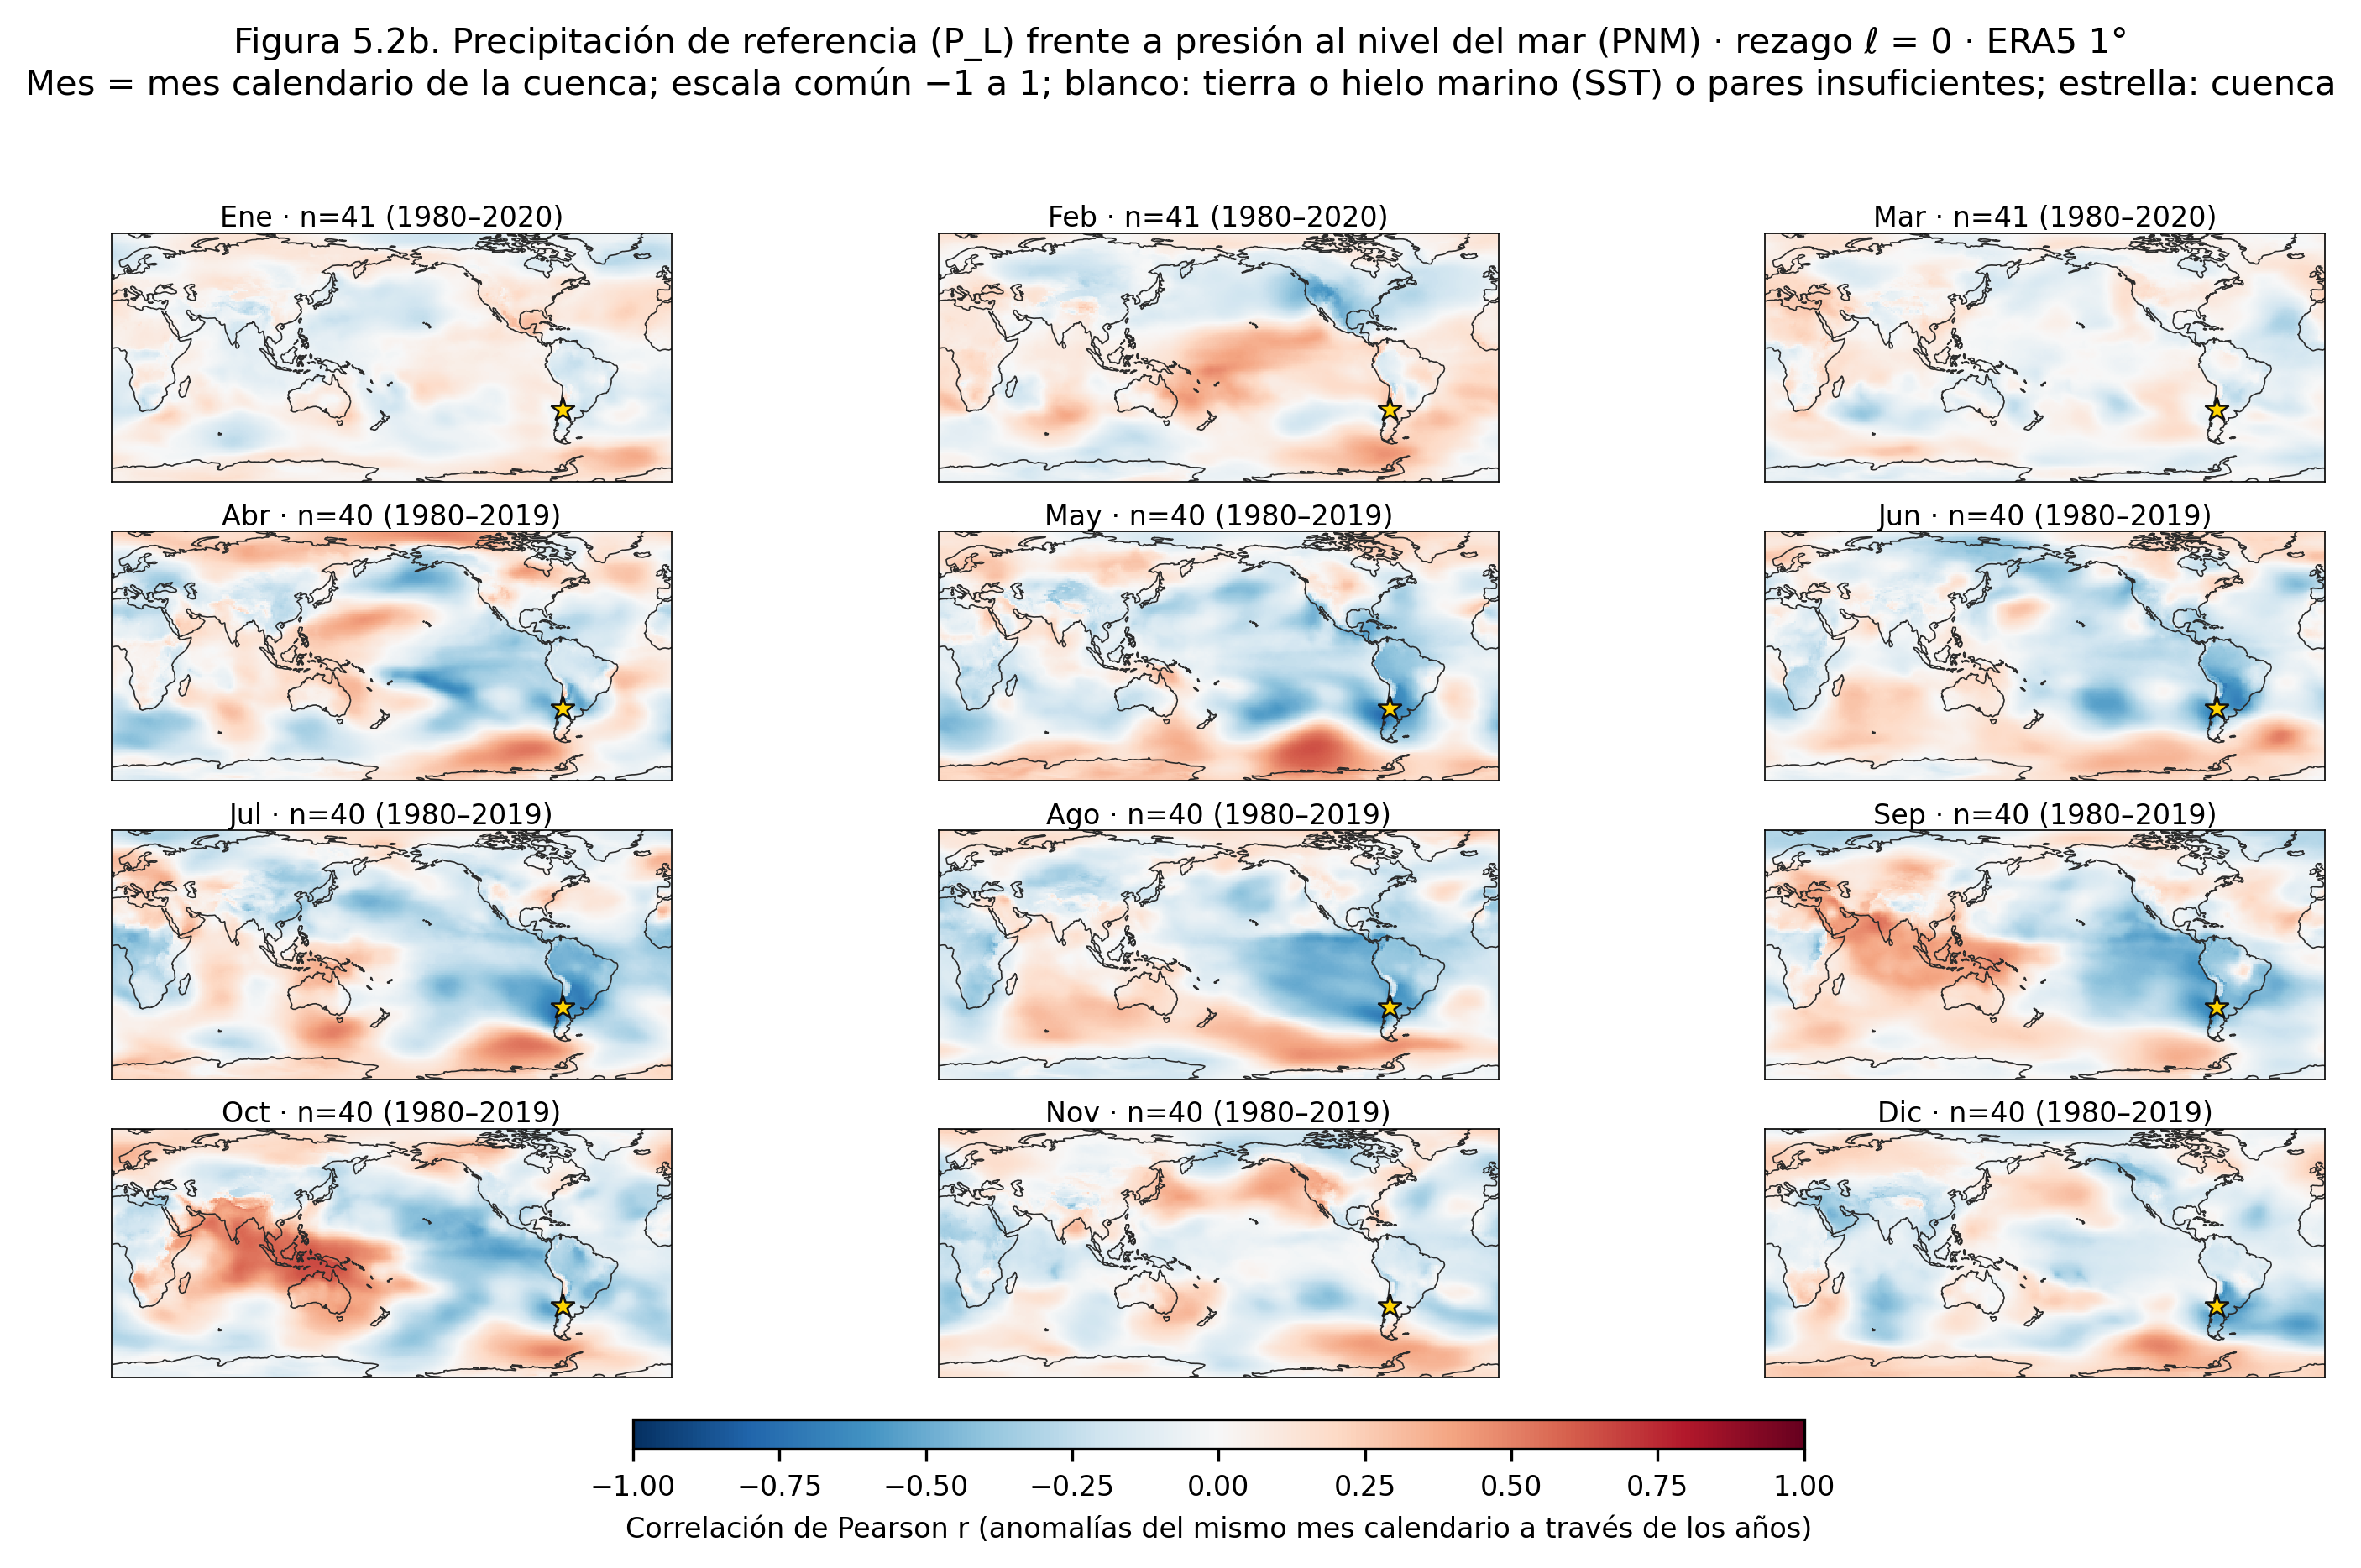
\includegraphics[width=\textwidth]{figura_5_2b_p_l_msl.png}
\caption{$P_L$ frente a PNM, $\ell=0$.}
\label{fig:pl_msl}
\end{figure}

\begin{figure}[H]
\centering
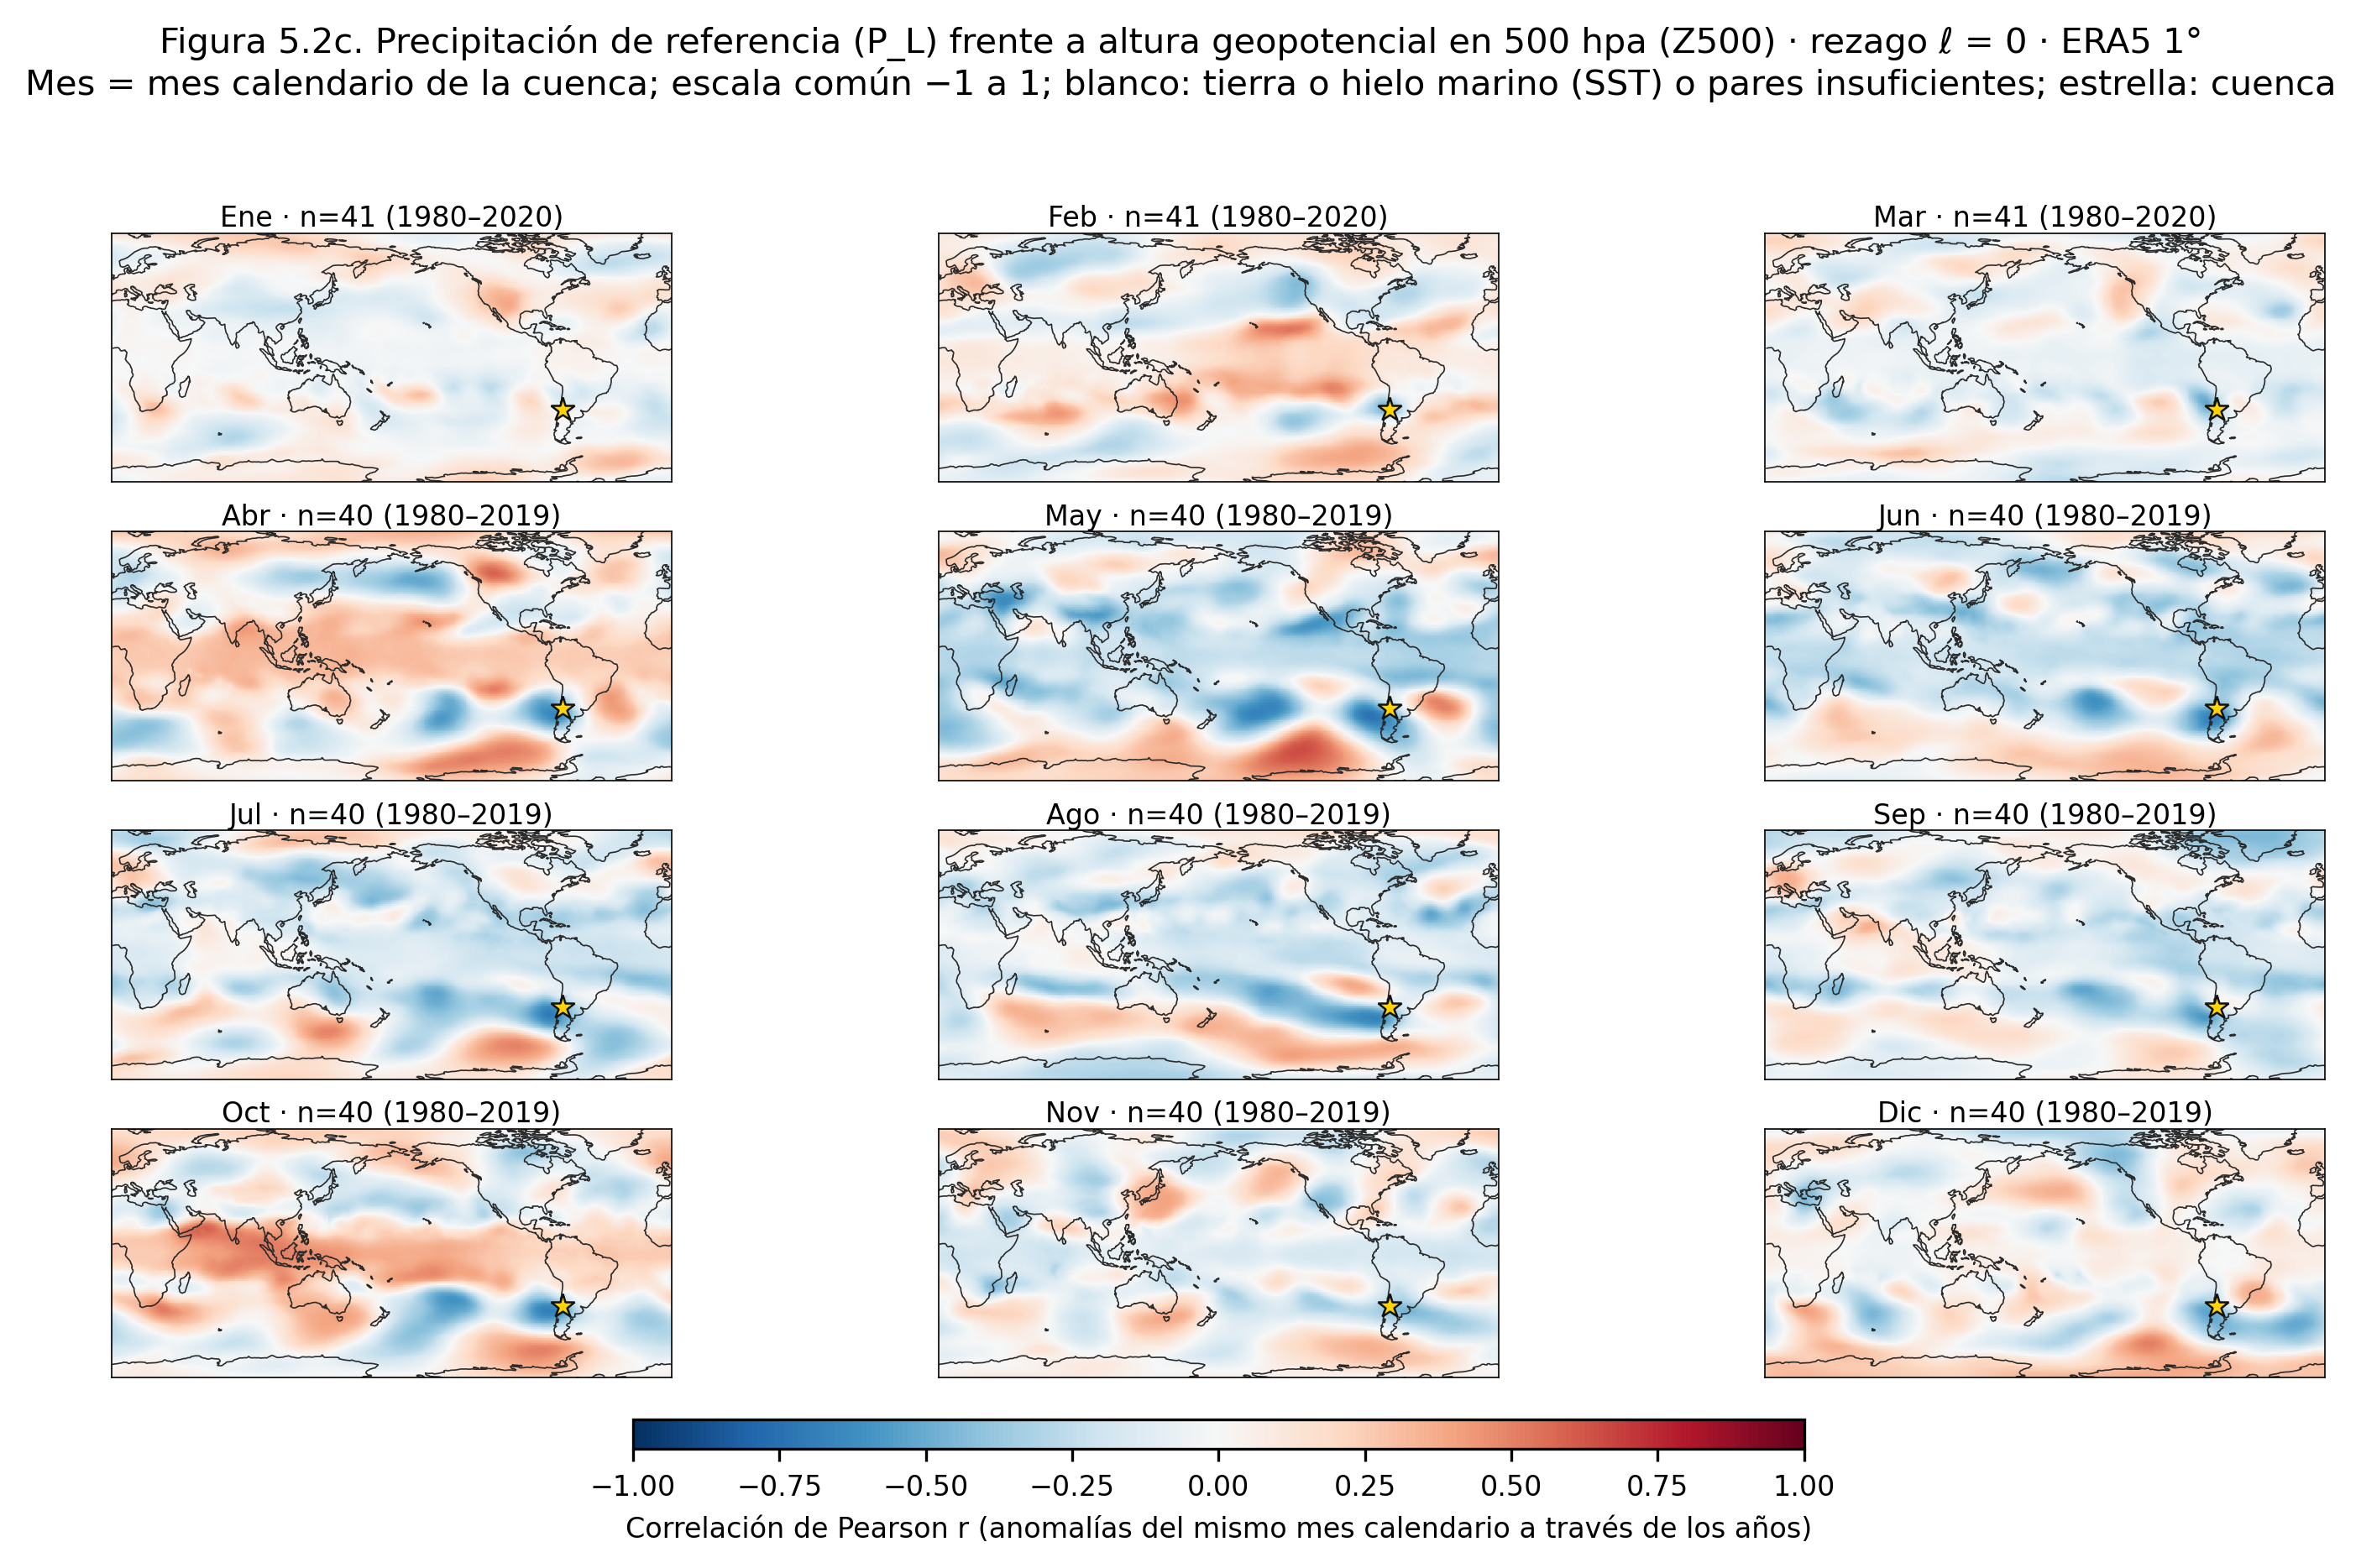
\includegraphics[width=\textwidth]{figura_5_2c_p_l_z500.png}
\caption{$P_L$ frente a Z500, $\ell=0$.}
\label{fig:pl_z500}
\end{figure}

\begin{figure}[H]
\centering
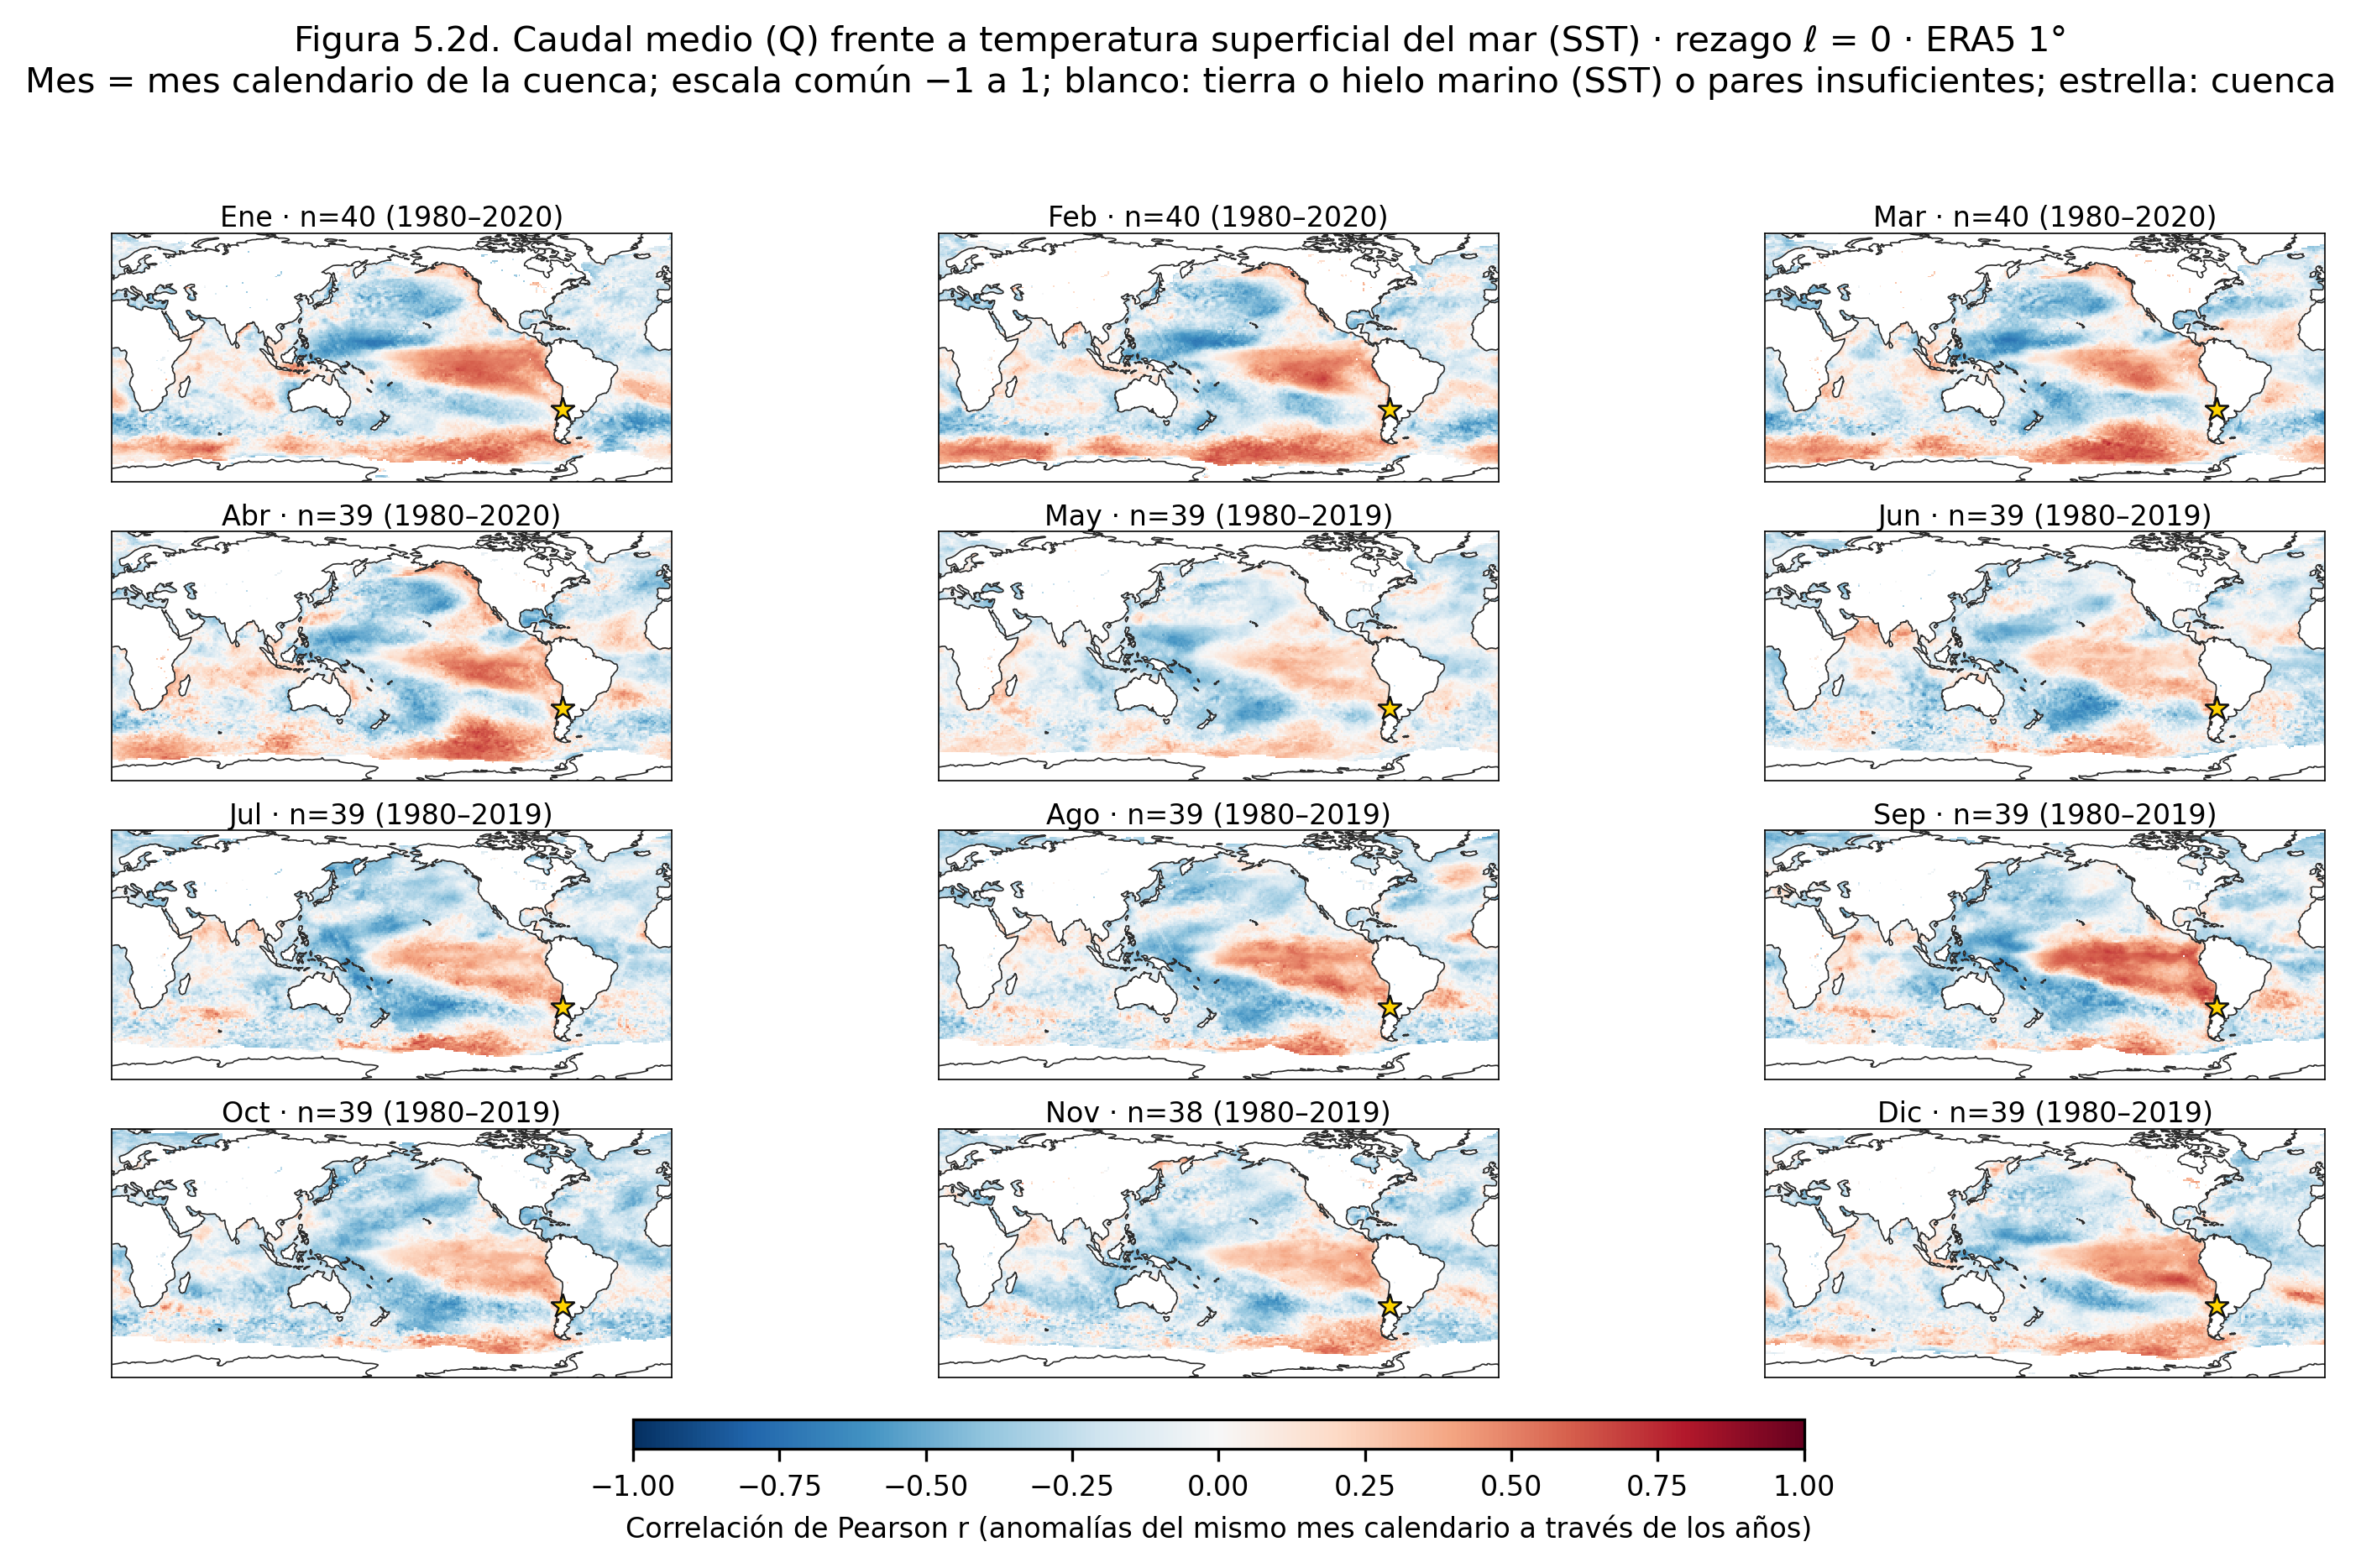
\includegraphics[width=\textwidth]{figura_5_2d_q_sst.png}
\caption{$Q$ frente a SST, $\ell=0$.}
\label{fig:q_sst}
\end{figure}

\begin{figure}[H]
\centering
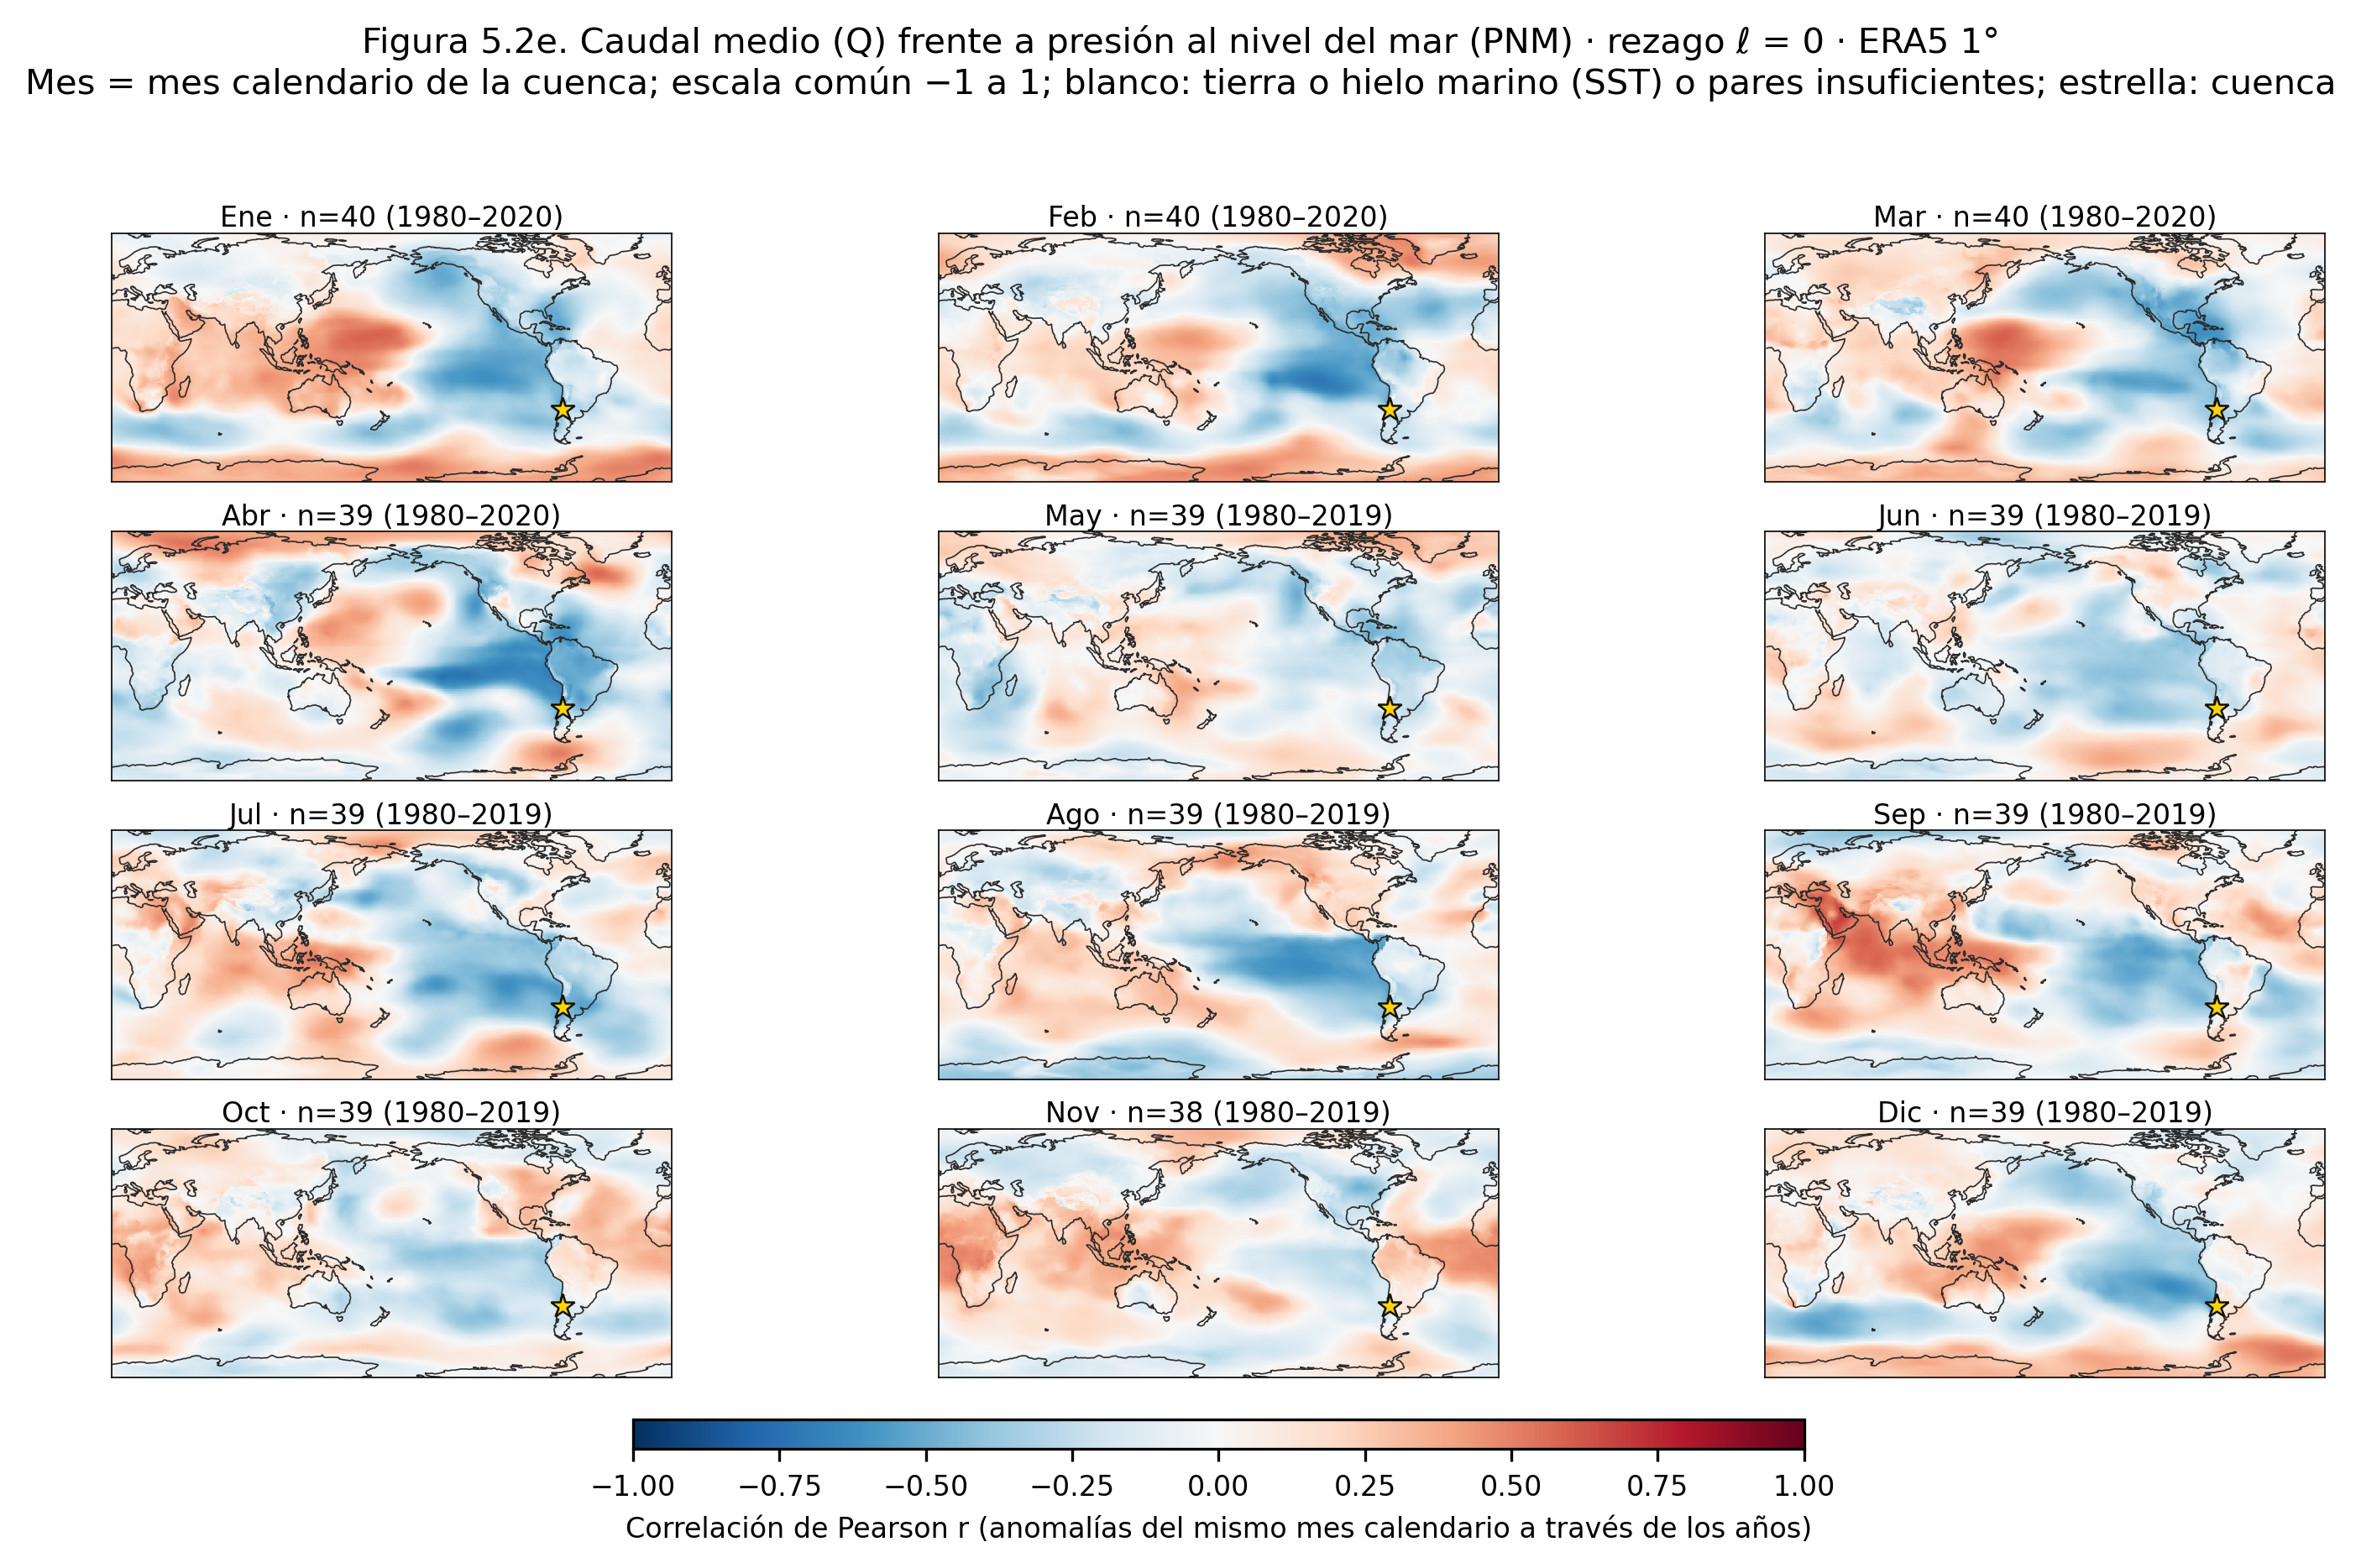
\includegraphics[width=\textwidth]{figura_5_2e_q_msl.png}
\caption{$Q$ frente a PNM, $\ell=0$.}
\label{fig:q_msl}
\end{figure}

\begin{figure}[H]
\centering
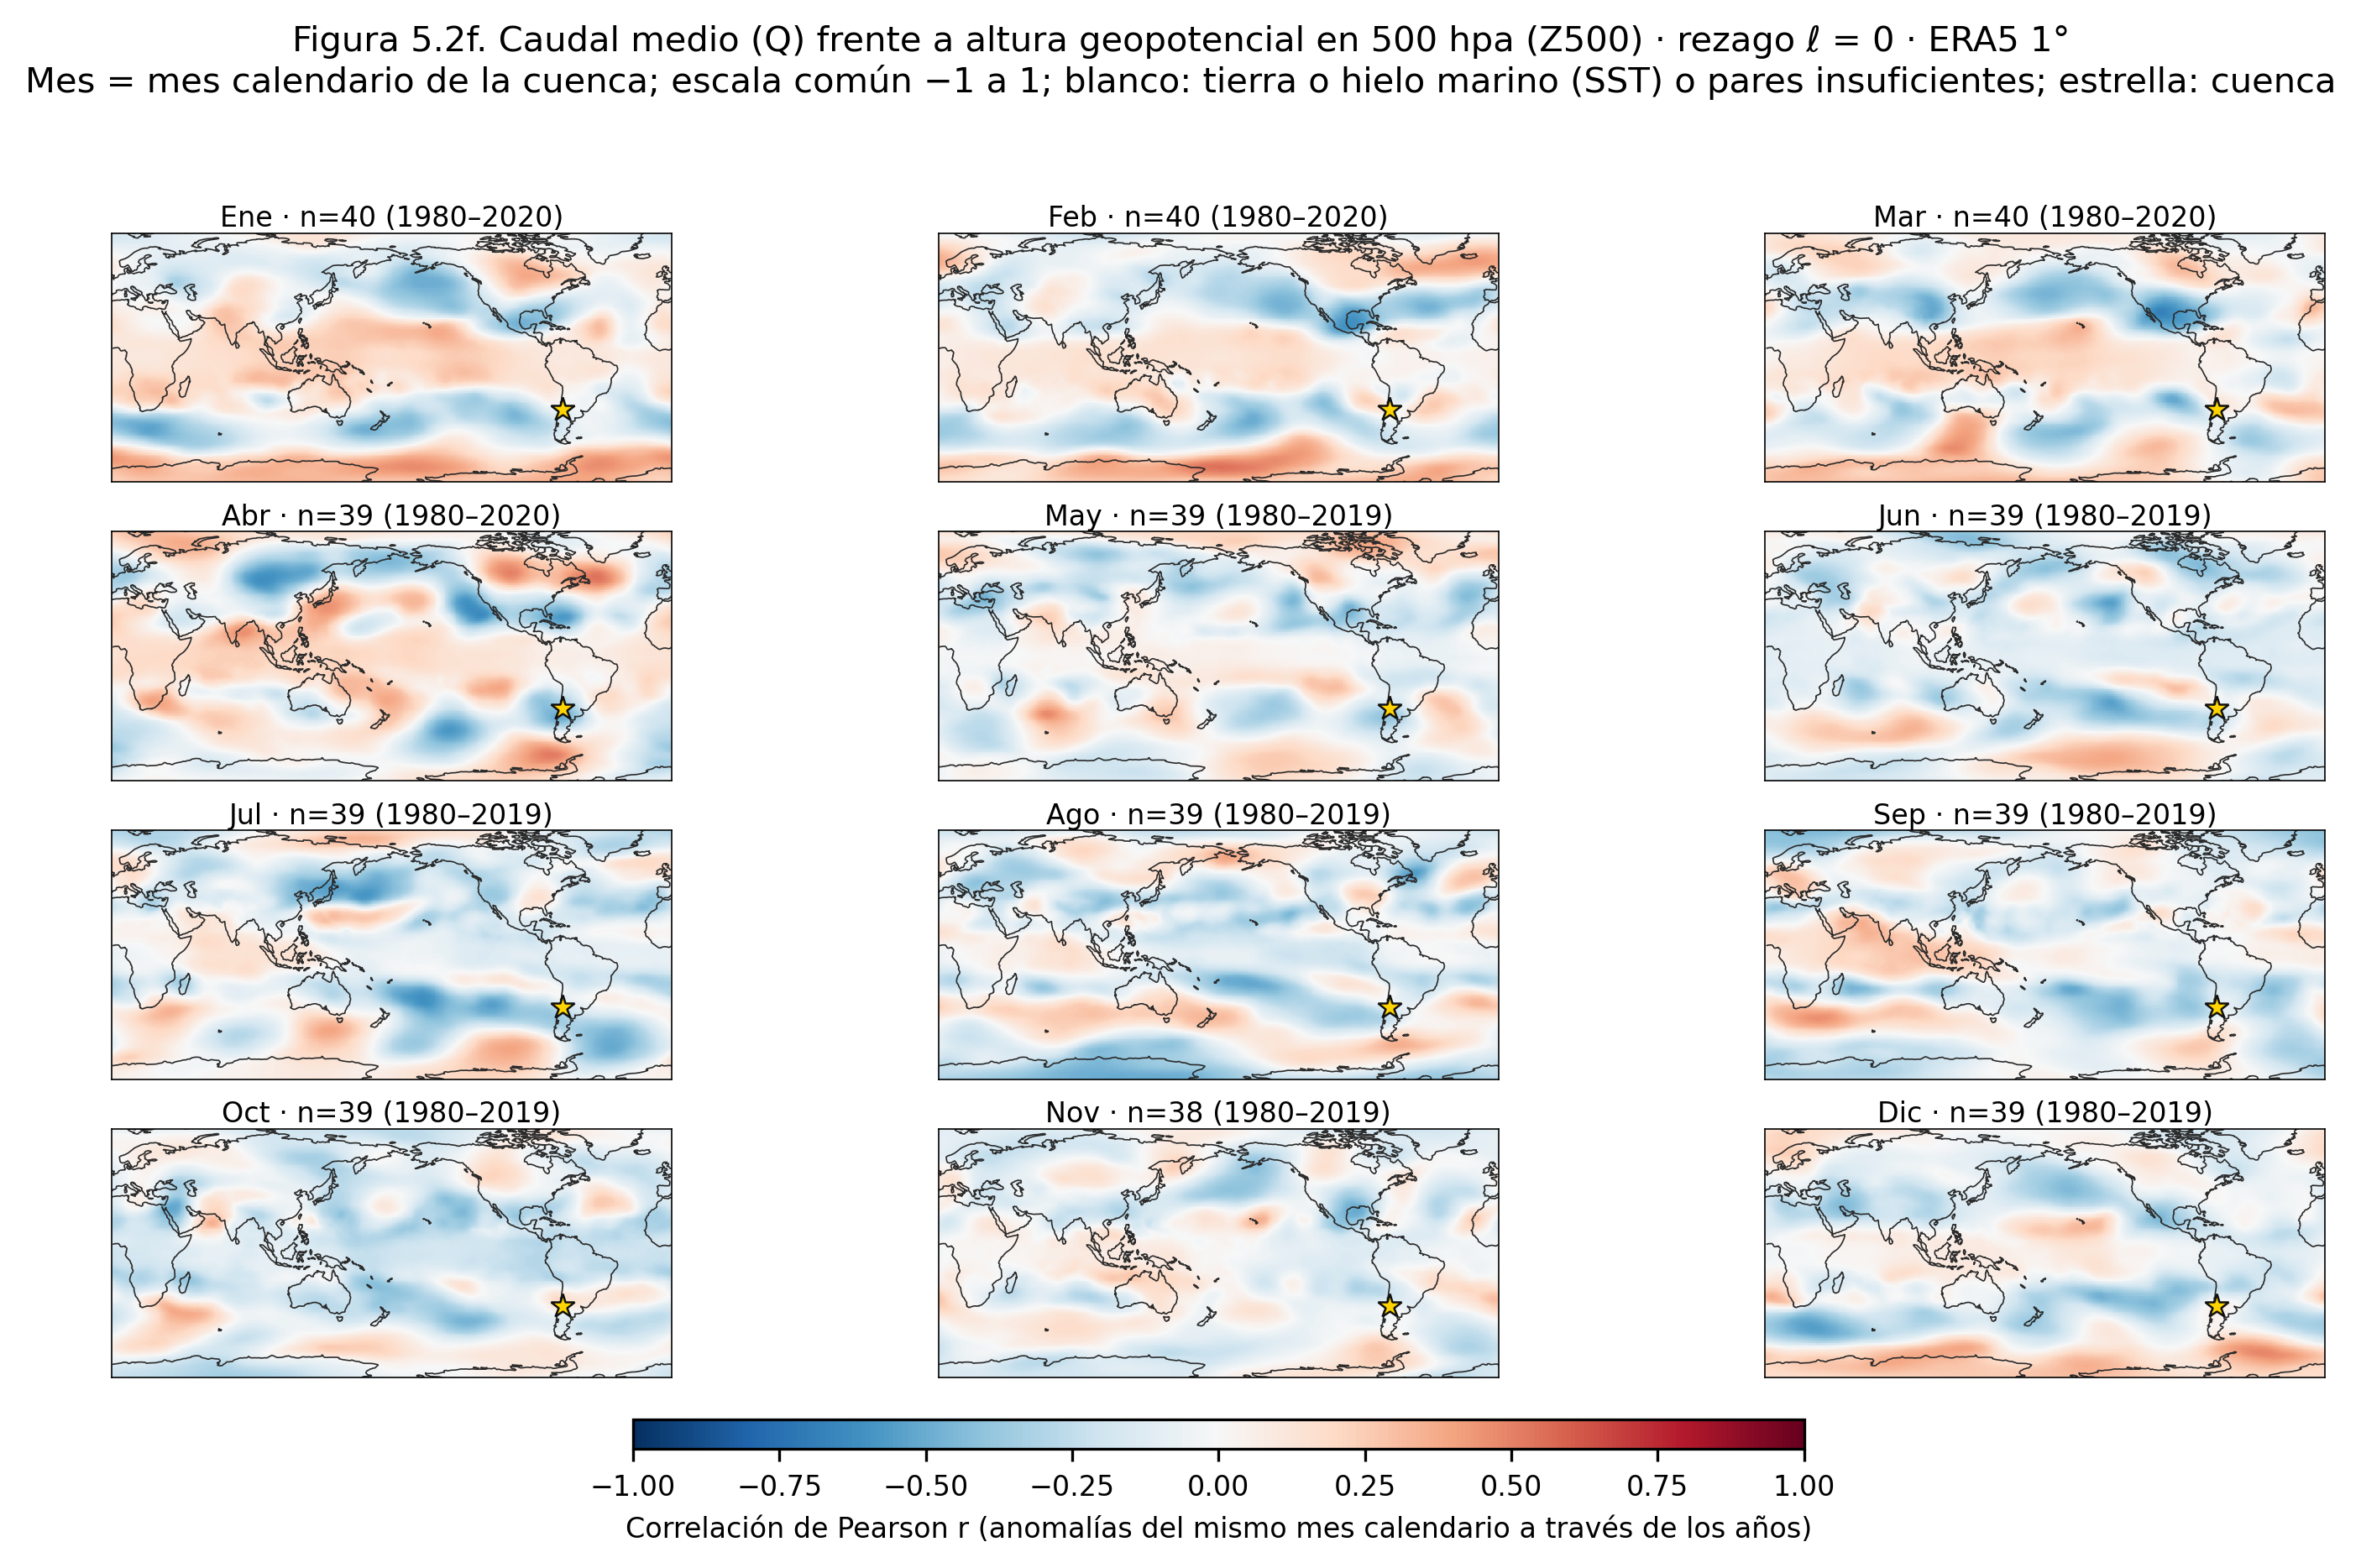
\includegraphics[width=\textwidth]{figura_5_2f_q_z500.png}
\caption{$Q$ frente a Z500, $\ell=0$.}
\label{fig:q_z500}
\end{figure}

\begin{figure}[H]
\centering
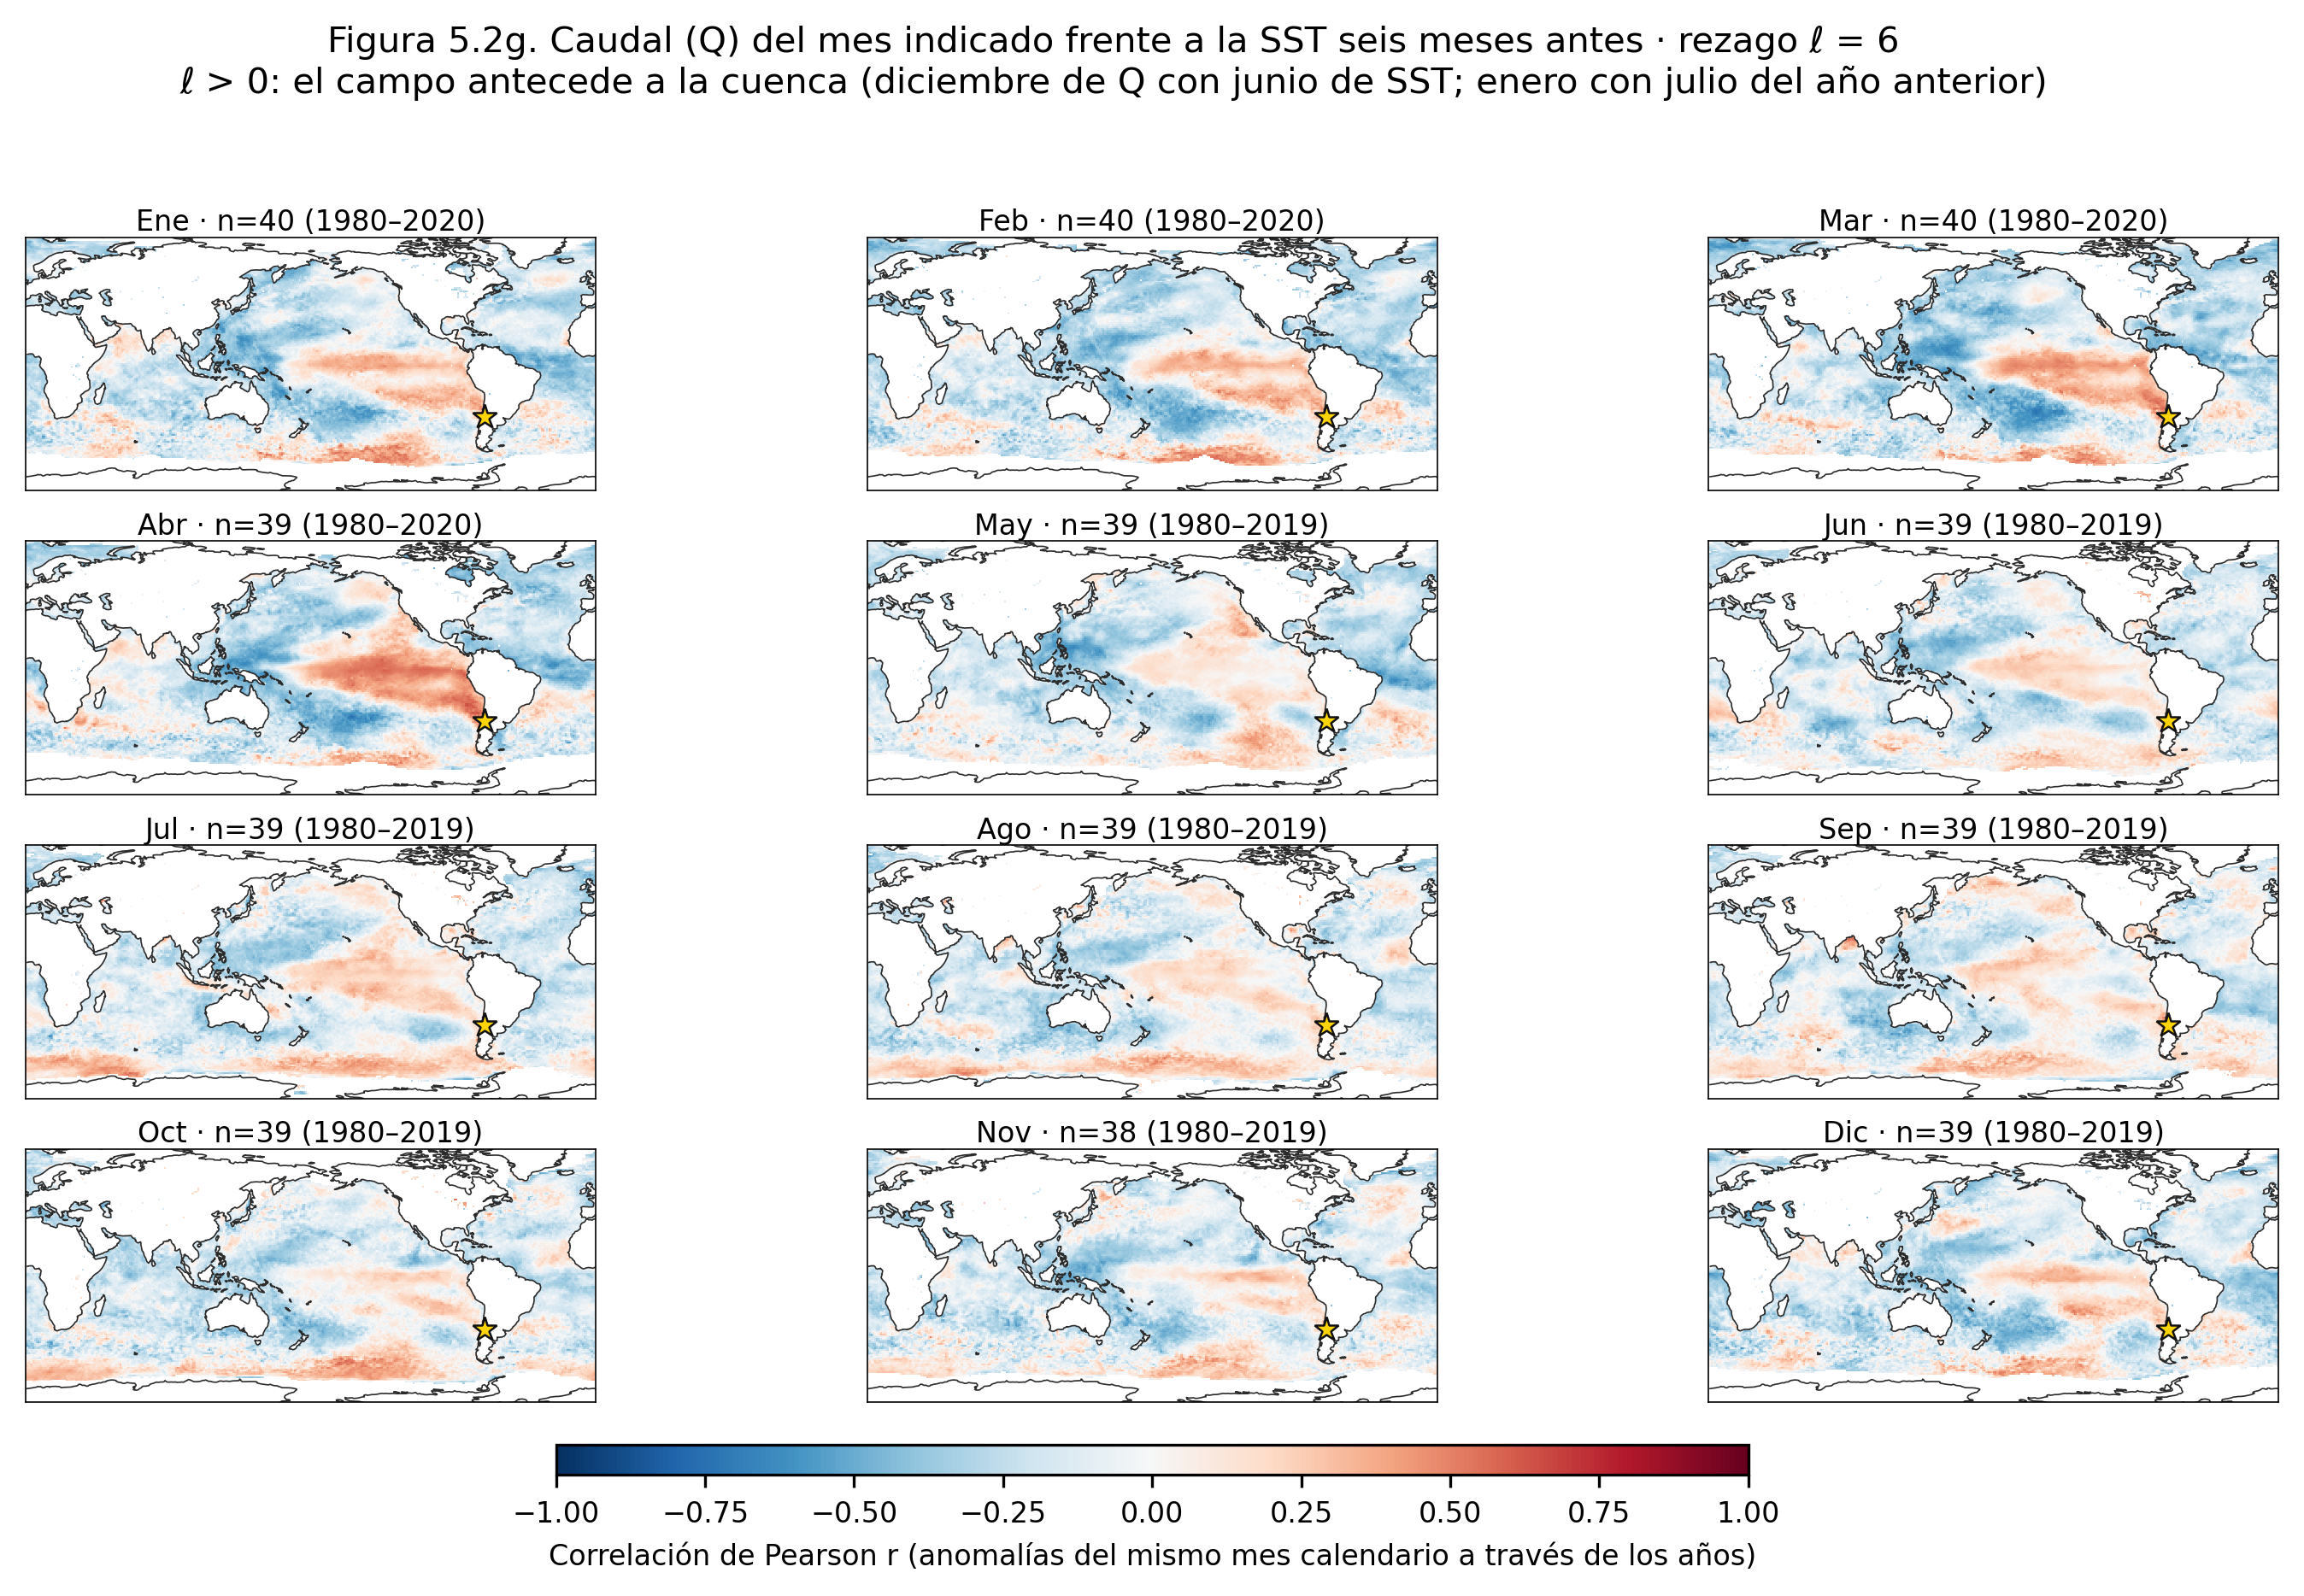
\includegraphics[width=\textwidth]{figura_5_2g_q_sst_rezago6.png}
\caption{$Q$ frente a la SST seis meses antes ($\ell=6$).}
\label{fig:lag6}
\end{figure}

\paragraph{Pearson frente a Spearman.} Como la lluvia mensual es muy asimétrica, se repitieron los mapas con
Spearman para la SST (Figura~\ref{fig:spear}). Los patrones casi no cambian: la correlación espacial entre los
mapas de Pearson y de Spearman va de 0.72 a 0.97 para $P_L$ y de 0.85 a 0.99 para $Q$, con una diferencia
mediana $|\Delta r|$ de 0.03--0.10. Los resultados no dependen de unos pocos meses extremos ni de una relación
monotónica no lineal.

\begin{figure}[H]
\centering
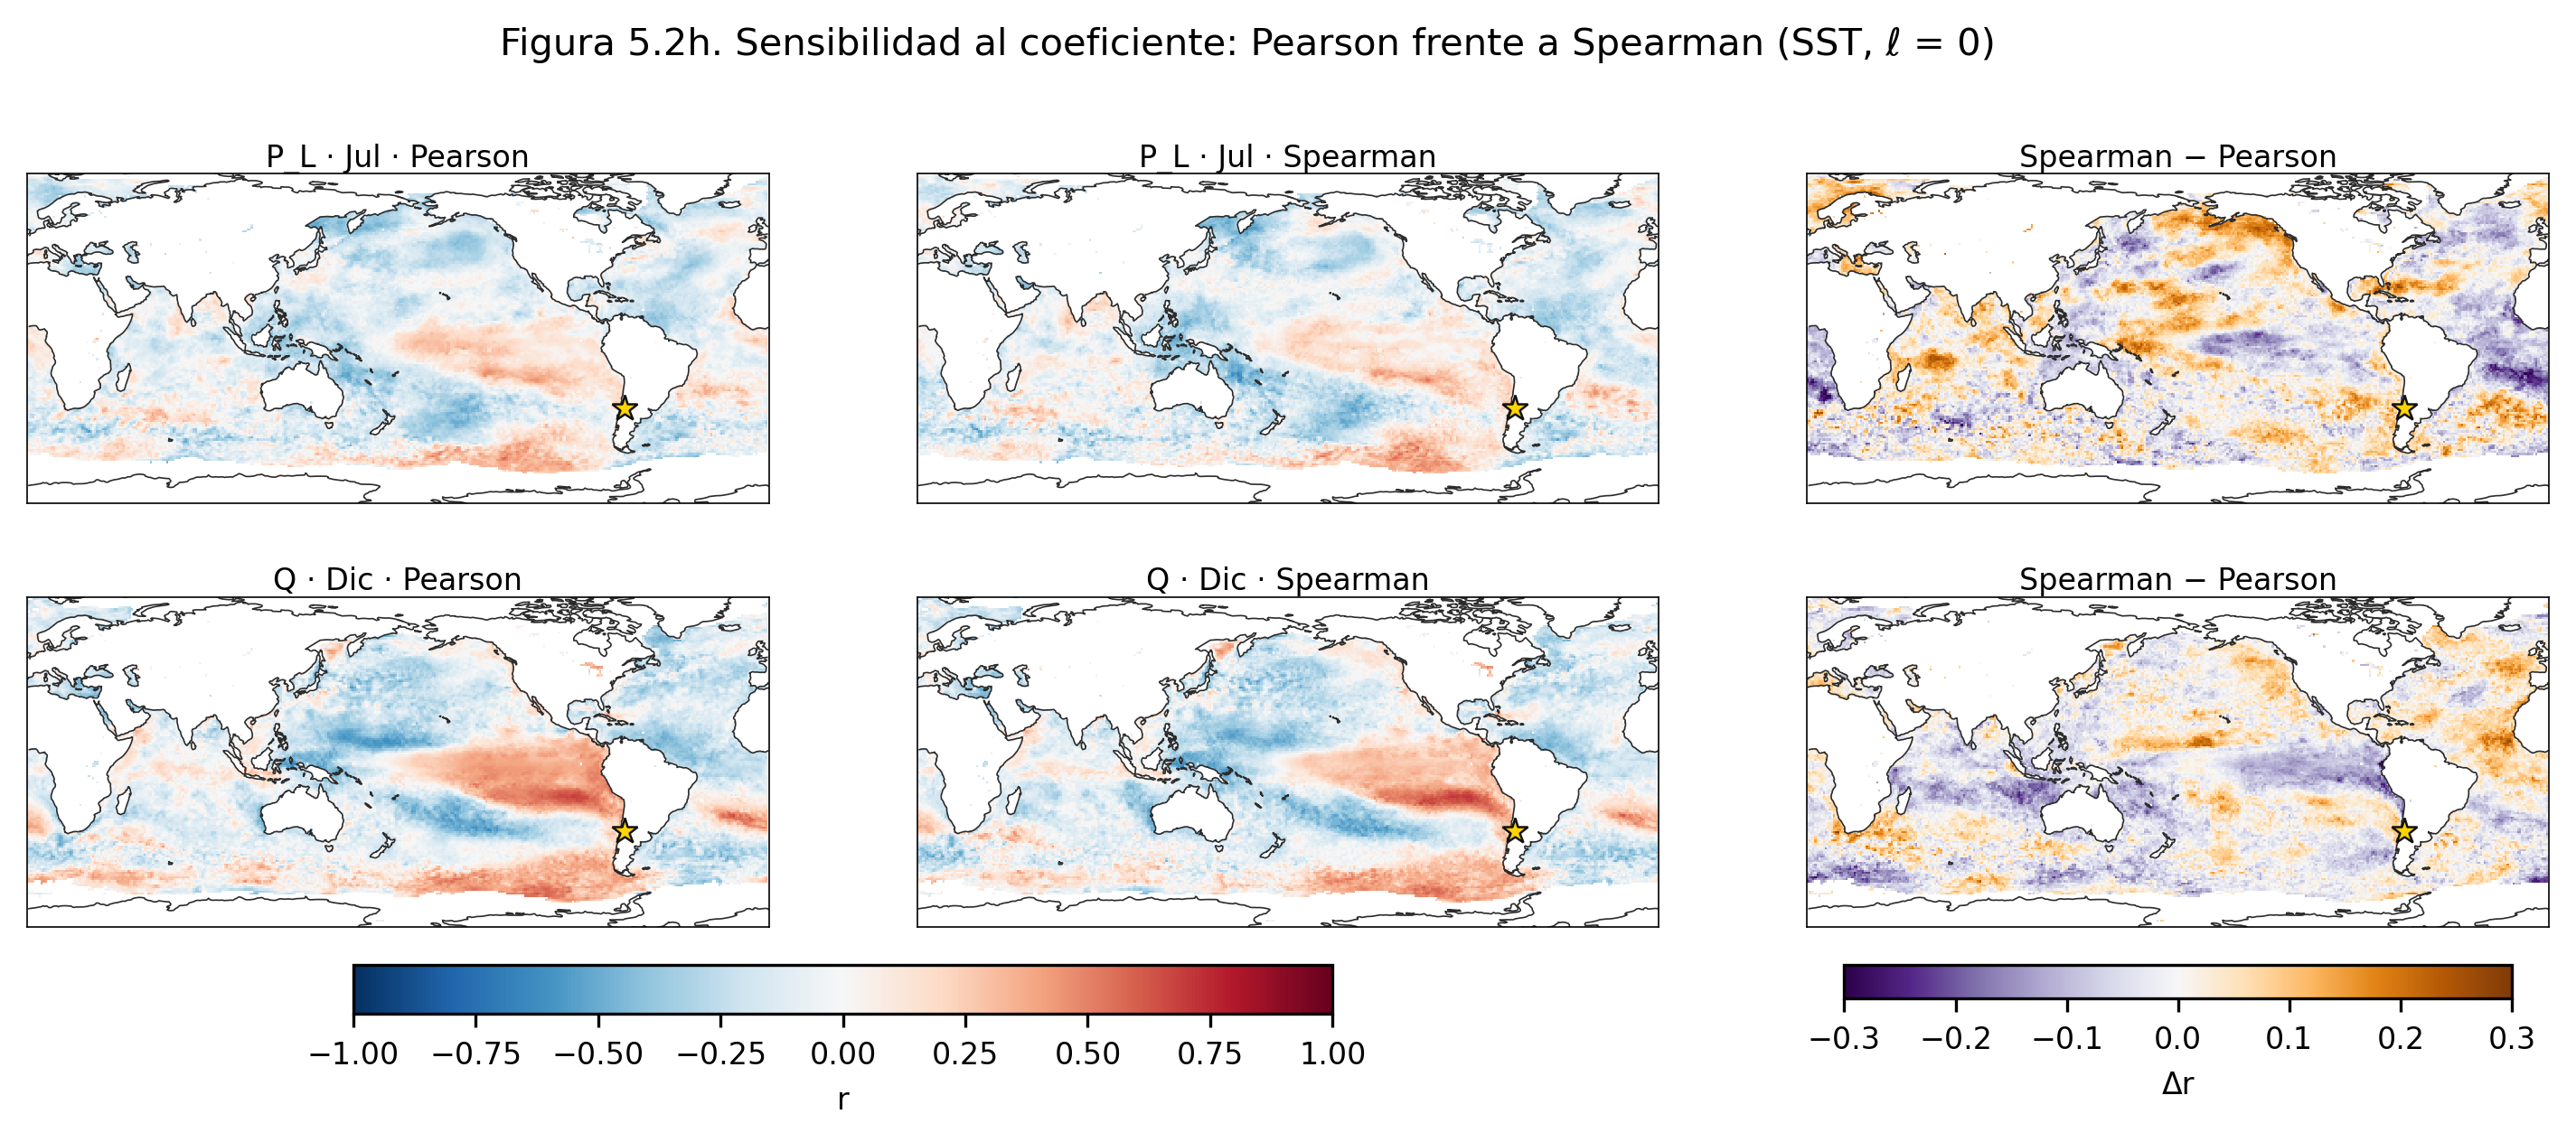
\includegraphics[width=\textwidth]{figura_5_2h_pearson_vs_spearman.png}
\caption{Pearson, Spearman y su diferencia para $P_L$ en julio y $Q$ en diciembre frente a la SST.}
\label{fig:spear}
\end{figure}

\section{Robustez (5.3)}
\label{sec:robustez}

\paragraph{Significancia y comparaciones múltiples.} En cada celda se aplicó una prueba $t$ con un tamaño de
muestra efectivo $n_\mathrm{eff}=n(1-r_{1x}r_{1y})/(1+r_{1x}r_{1y})$ \citep{Bretherton1999}, donde $r_1$ es la
autocorrelación entre años consecutivos de la subserie del mes. Esa es la dependencia relevante en un mapa de un
mes calendario, y resultó débil ($n_\mathrm{eff}$ mediano de 39--40 para $n=38$--41). La familia de pruebas es
el conjunto de celdas válidas de \emph{un} mapa, y el control es FDR de Benjamini--Hochberg con
$\alpha_\mathrm{FDR}=0.10$, que equivale aproximadamente a $\alpha_\mathrm{global}=0.05$ en campos
espacialmente correlacionados \citep{BH1995,Wilks2016}. Una celda requiere al menos 15 años, y se excluyen las
celdas con algún año enmascarado (hielo). El supuesto de FDR de dependencia positiva entre pruebas es razonable
para campos suaves, pero los 12 meses y las 6 combinaciones siguen siendo muchas familias; por eso se exige un
\emph{patrón espacial coherente} y no píxeles aislados (Figura~\ref{fig:fdr}).

\begin{figure}[H]
\centering
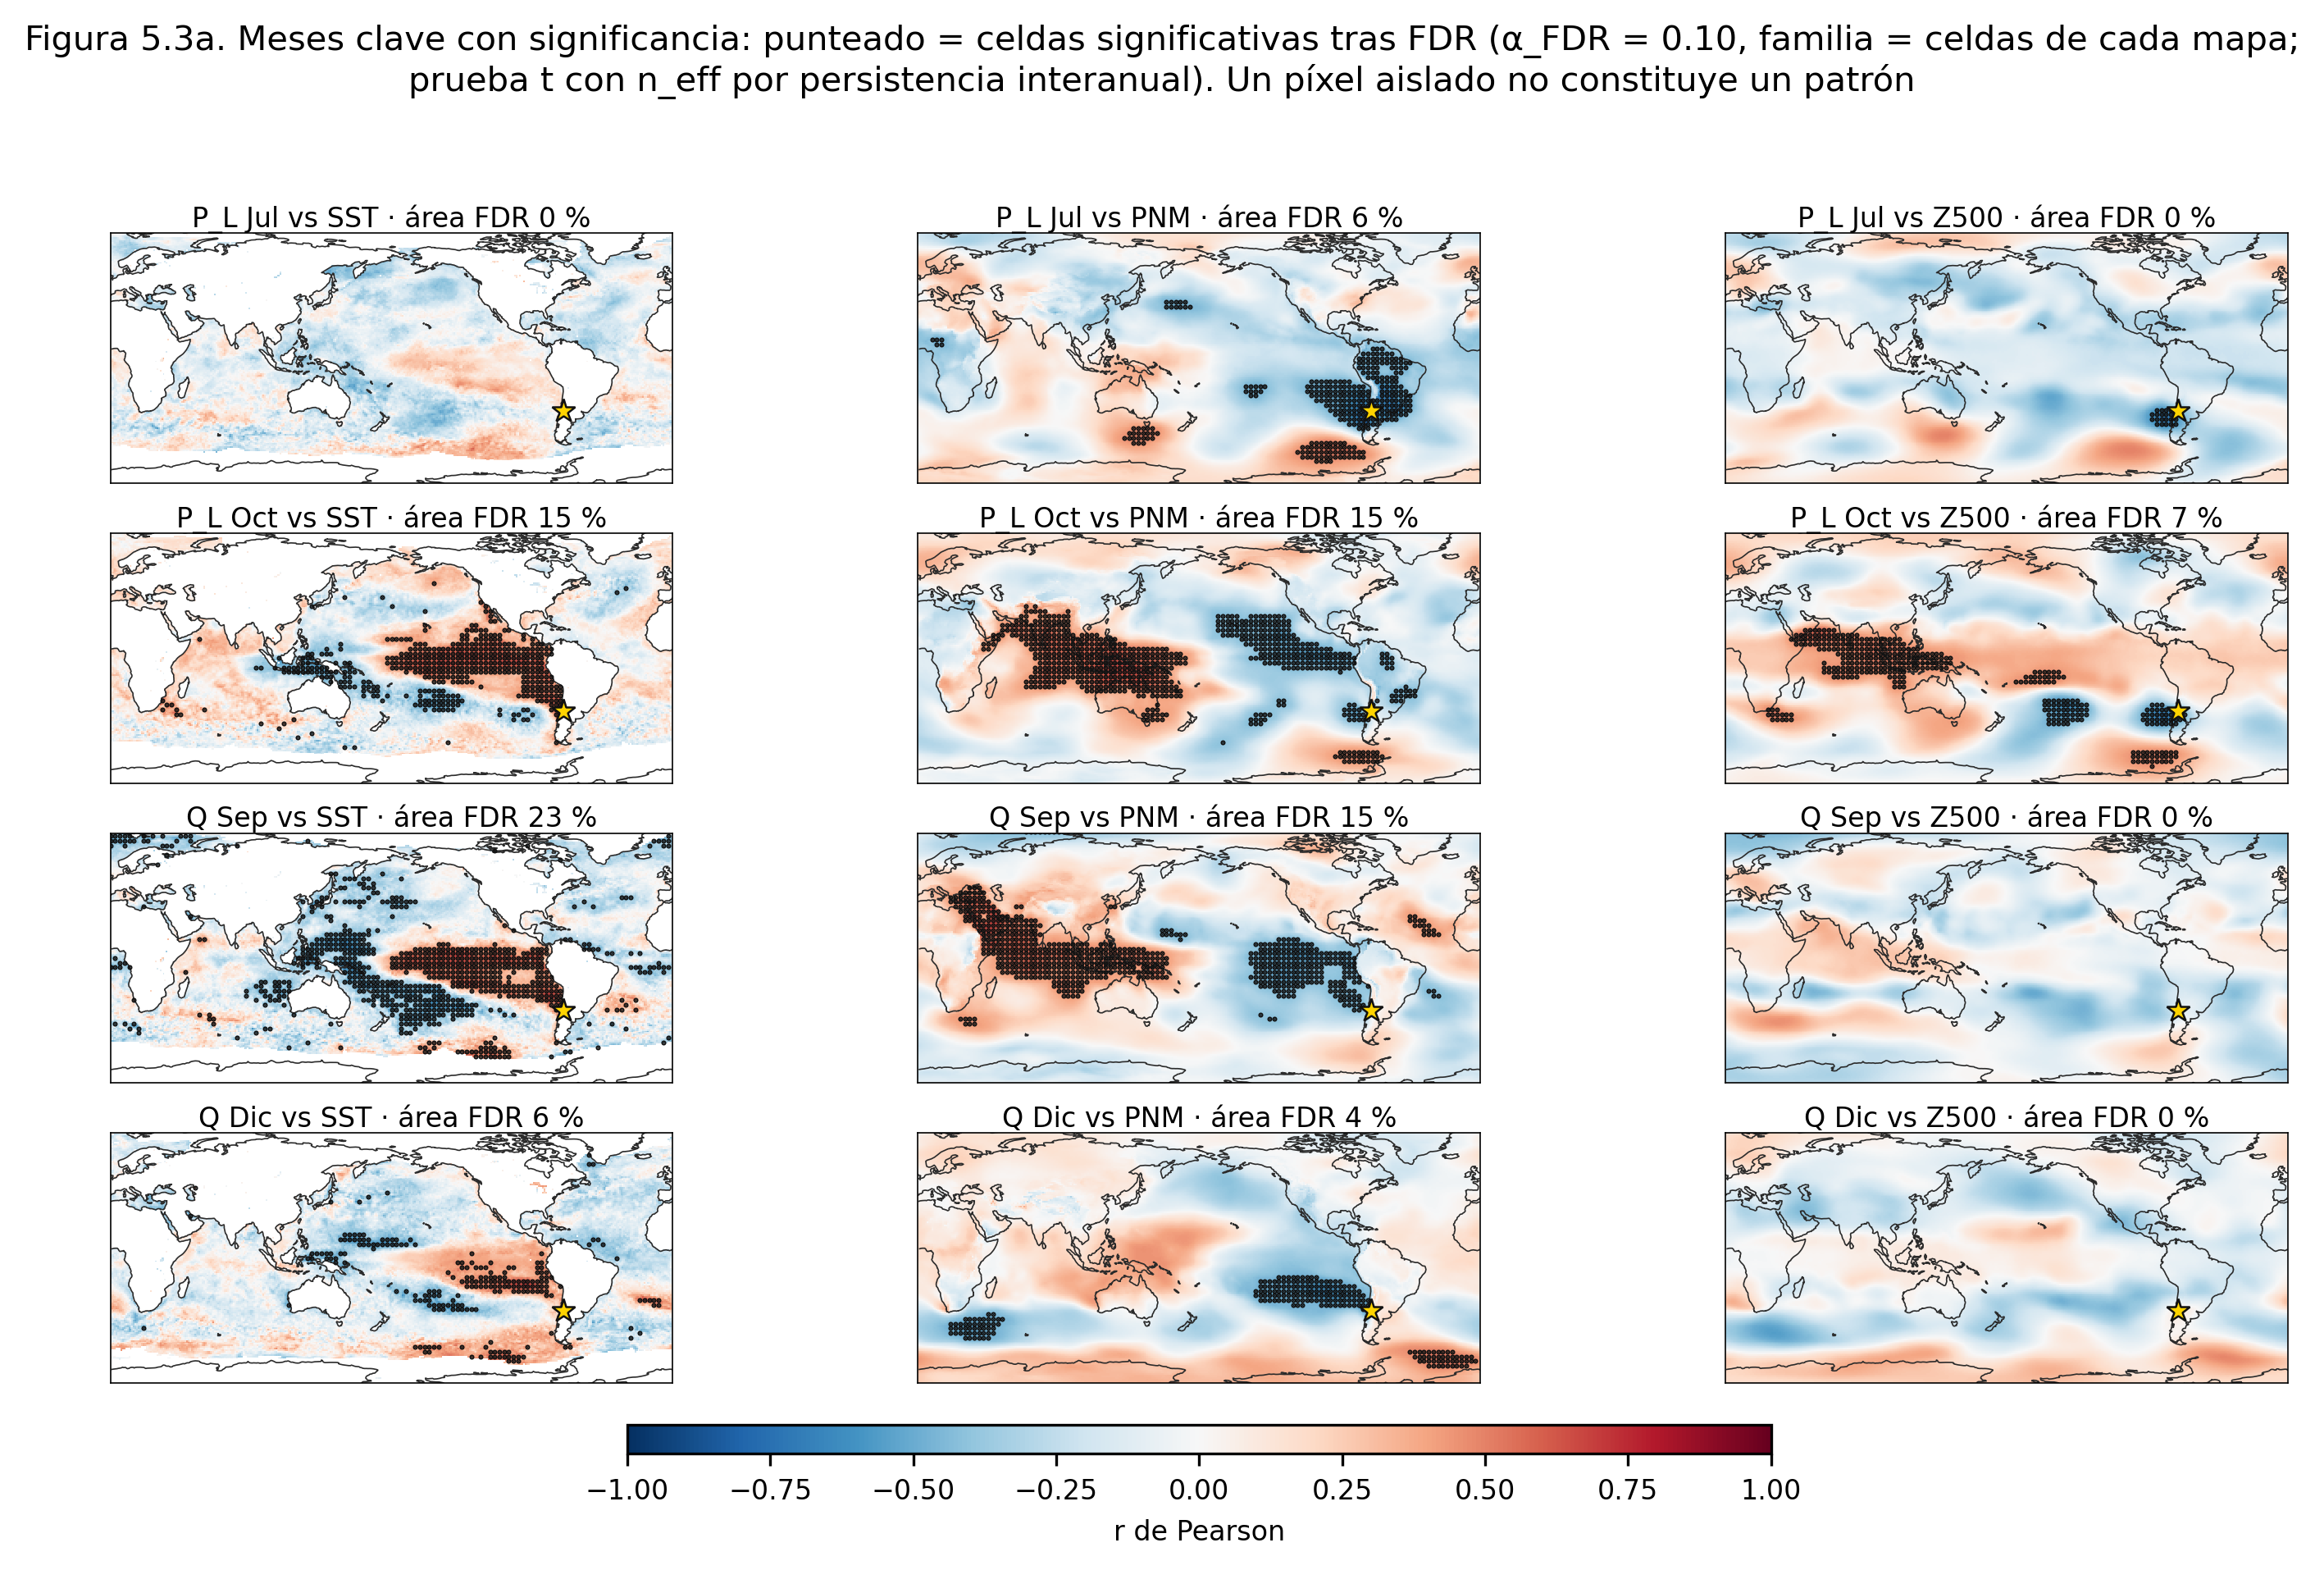
\includegraphics[width=\textwidth]{figura_5_3a_significancia_fdr.png}
\caption{Meses clave con punteado de las celdas significativas tras FDR. Script \texttt{18\_p5\_3\_robustez.py}.}
\label{fig:fdr}
\end{figure}

La fracción del área con significancia tras FDR es baja para $P_L$ frente a la SST (media de 2\,\%, máxima de
15\,\% en octubre). Es mayor frente a la PNM (máxima de 15\,\%) y en $Q$ frente a la SST (media de 10\,\%,
máxima de 23\,\%). Con 40 años, una correlación de 0.4 apenas supera el umbral local, y el FDR es exigente: la
ausencia de punteado no implica ausencia de asociación. Al agrupar las anomalías de todos los meses ($n\approx480$,
Figura~\ref{fig:todos}) emergen con claridad tres patrones: la ``herradura'' de ENSO en la SST para $Q$; un
patrón de tipo Oscilación del Sur en la PNM para $Q$ (positivo sobre Indonesia y Australia, negativo sobre el
Pacífico central y oriental); y para $P_L$ un dipolo de PNM con un centro negativo frente a Chile central y
uno positivo sobre los mares de Amundsen y Bellingshausen.

\begin{figure}[H]
\centering
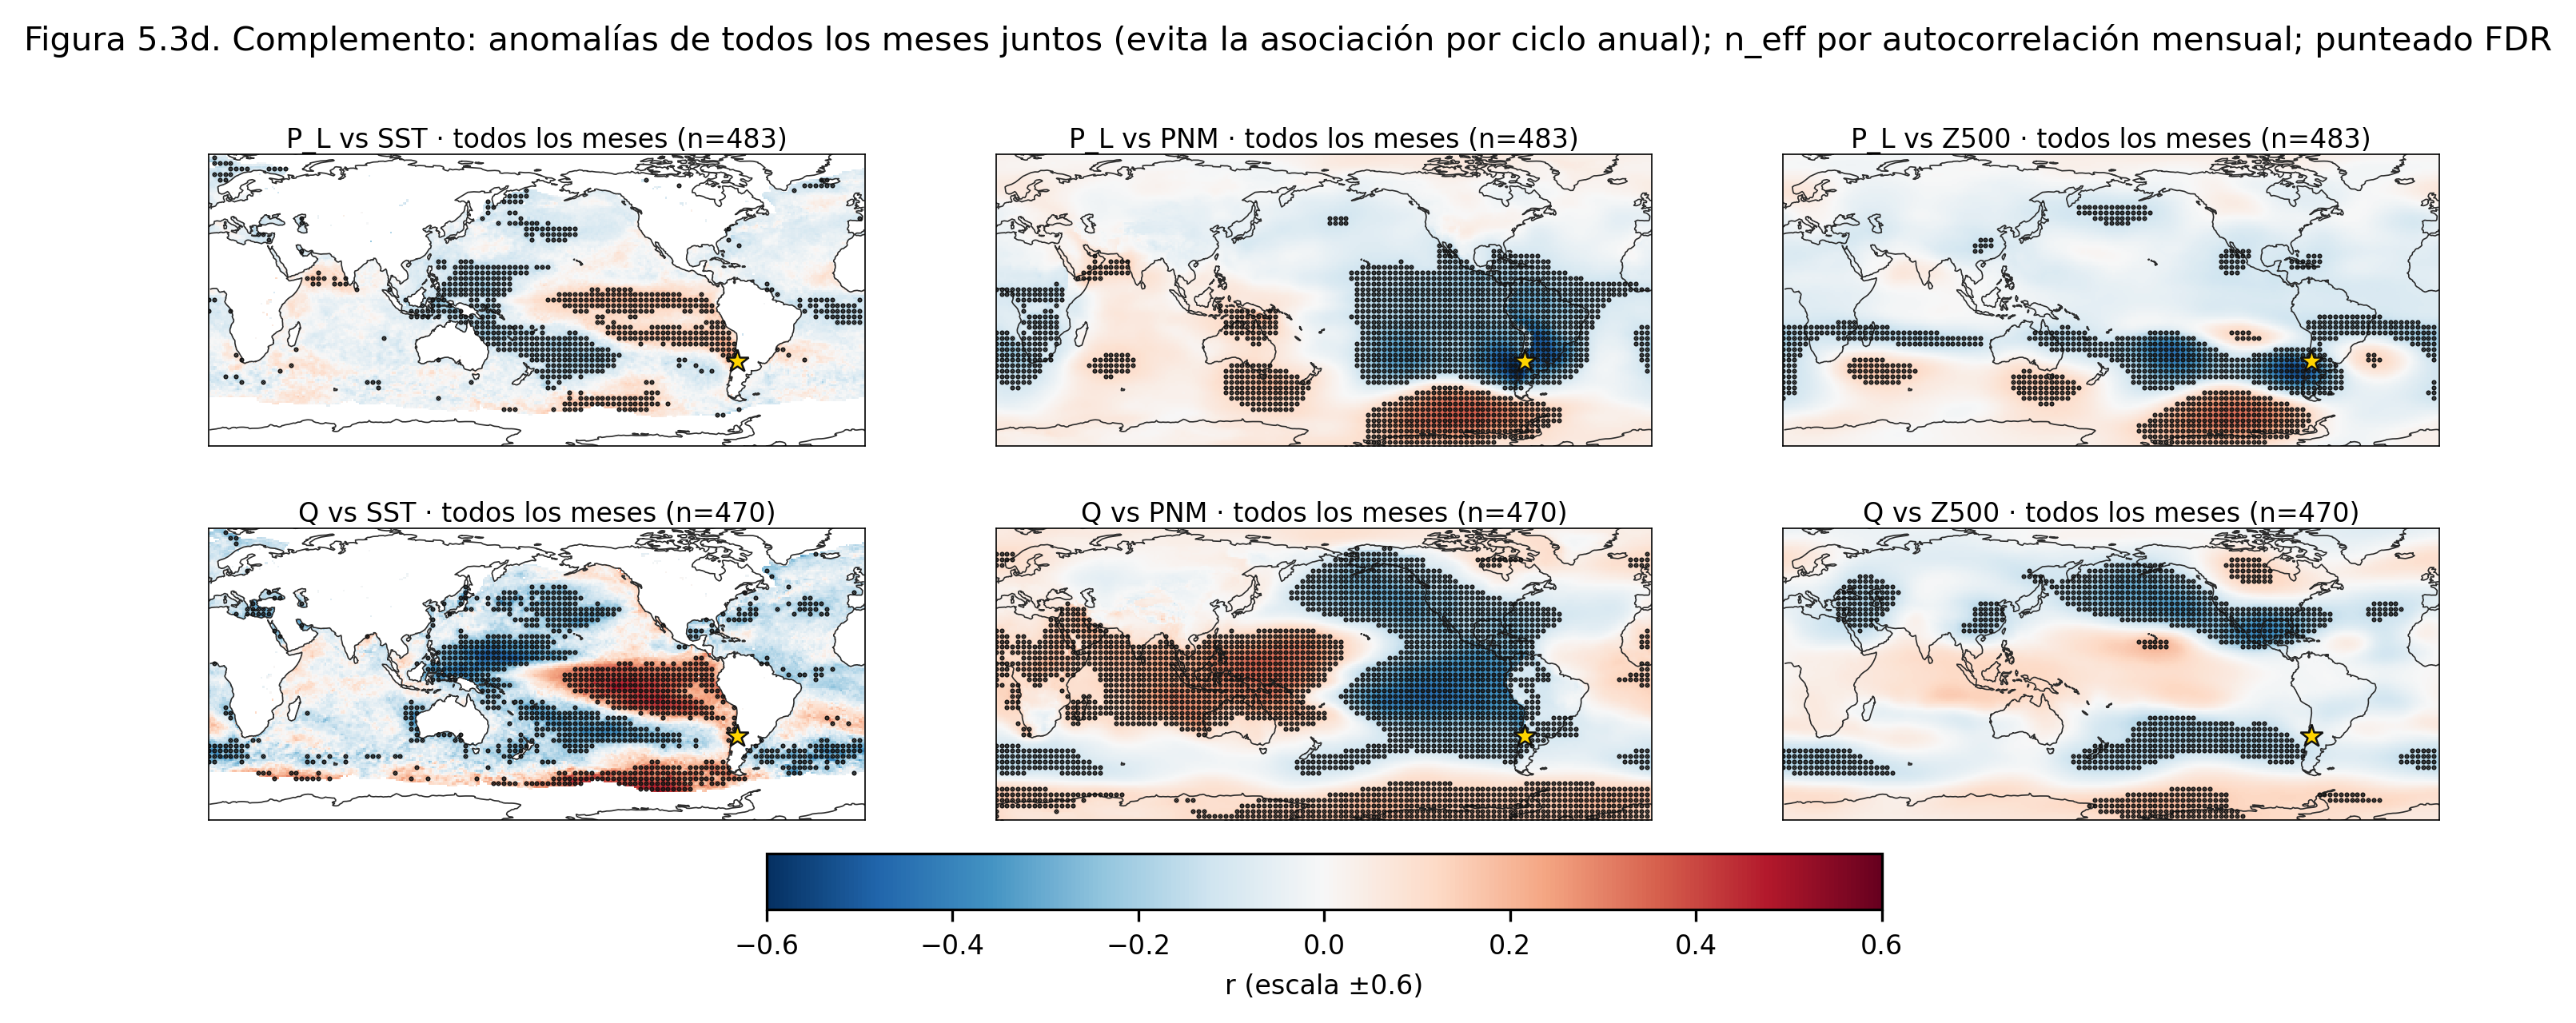
\includegraphics[width=\textwidth]{figura_5_3d_todos_los_meses.png}
\caption{Correlación con las anomalías de todos los meses juntos (sin ciclo anual compartido) y punteado FDR.}
\label{fig:todos}
\end{figure}

\paragraph{Anomalías frente a series sin tendencia.} Se retiró la tendencia lineal en el año de ambas series,
por mes calendario y celda (Figura~\ref{fig:tend}). Los patrones casi no cambian: la correlación espacial entre
los mapas con y sin tendencia tiene mediana de 0.89--0.99. Para $Q$, la asociación con Niño 3.4 incluso
aumenta (enero: de 0.45 a 0.50; marzo: de 0.35 a 0.44). La tendencia negativa del caudal (punto 3) no produce
estas correlaciones; más bien enmascara parte de la asociación interanual con ENSO.

\begin{figure}[H]
\centering
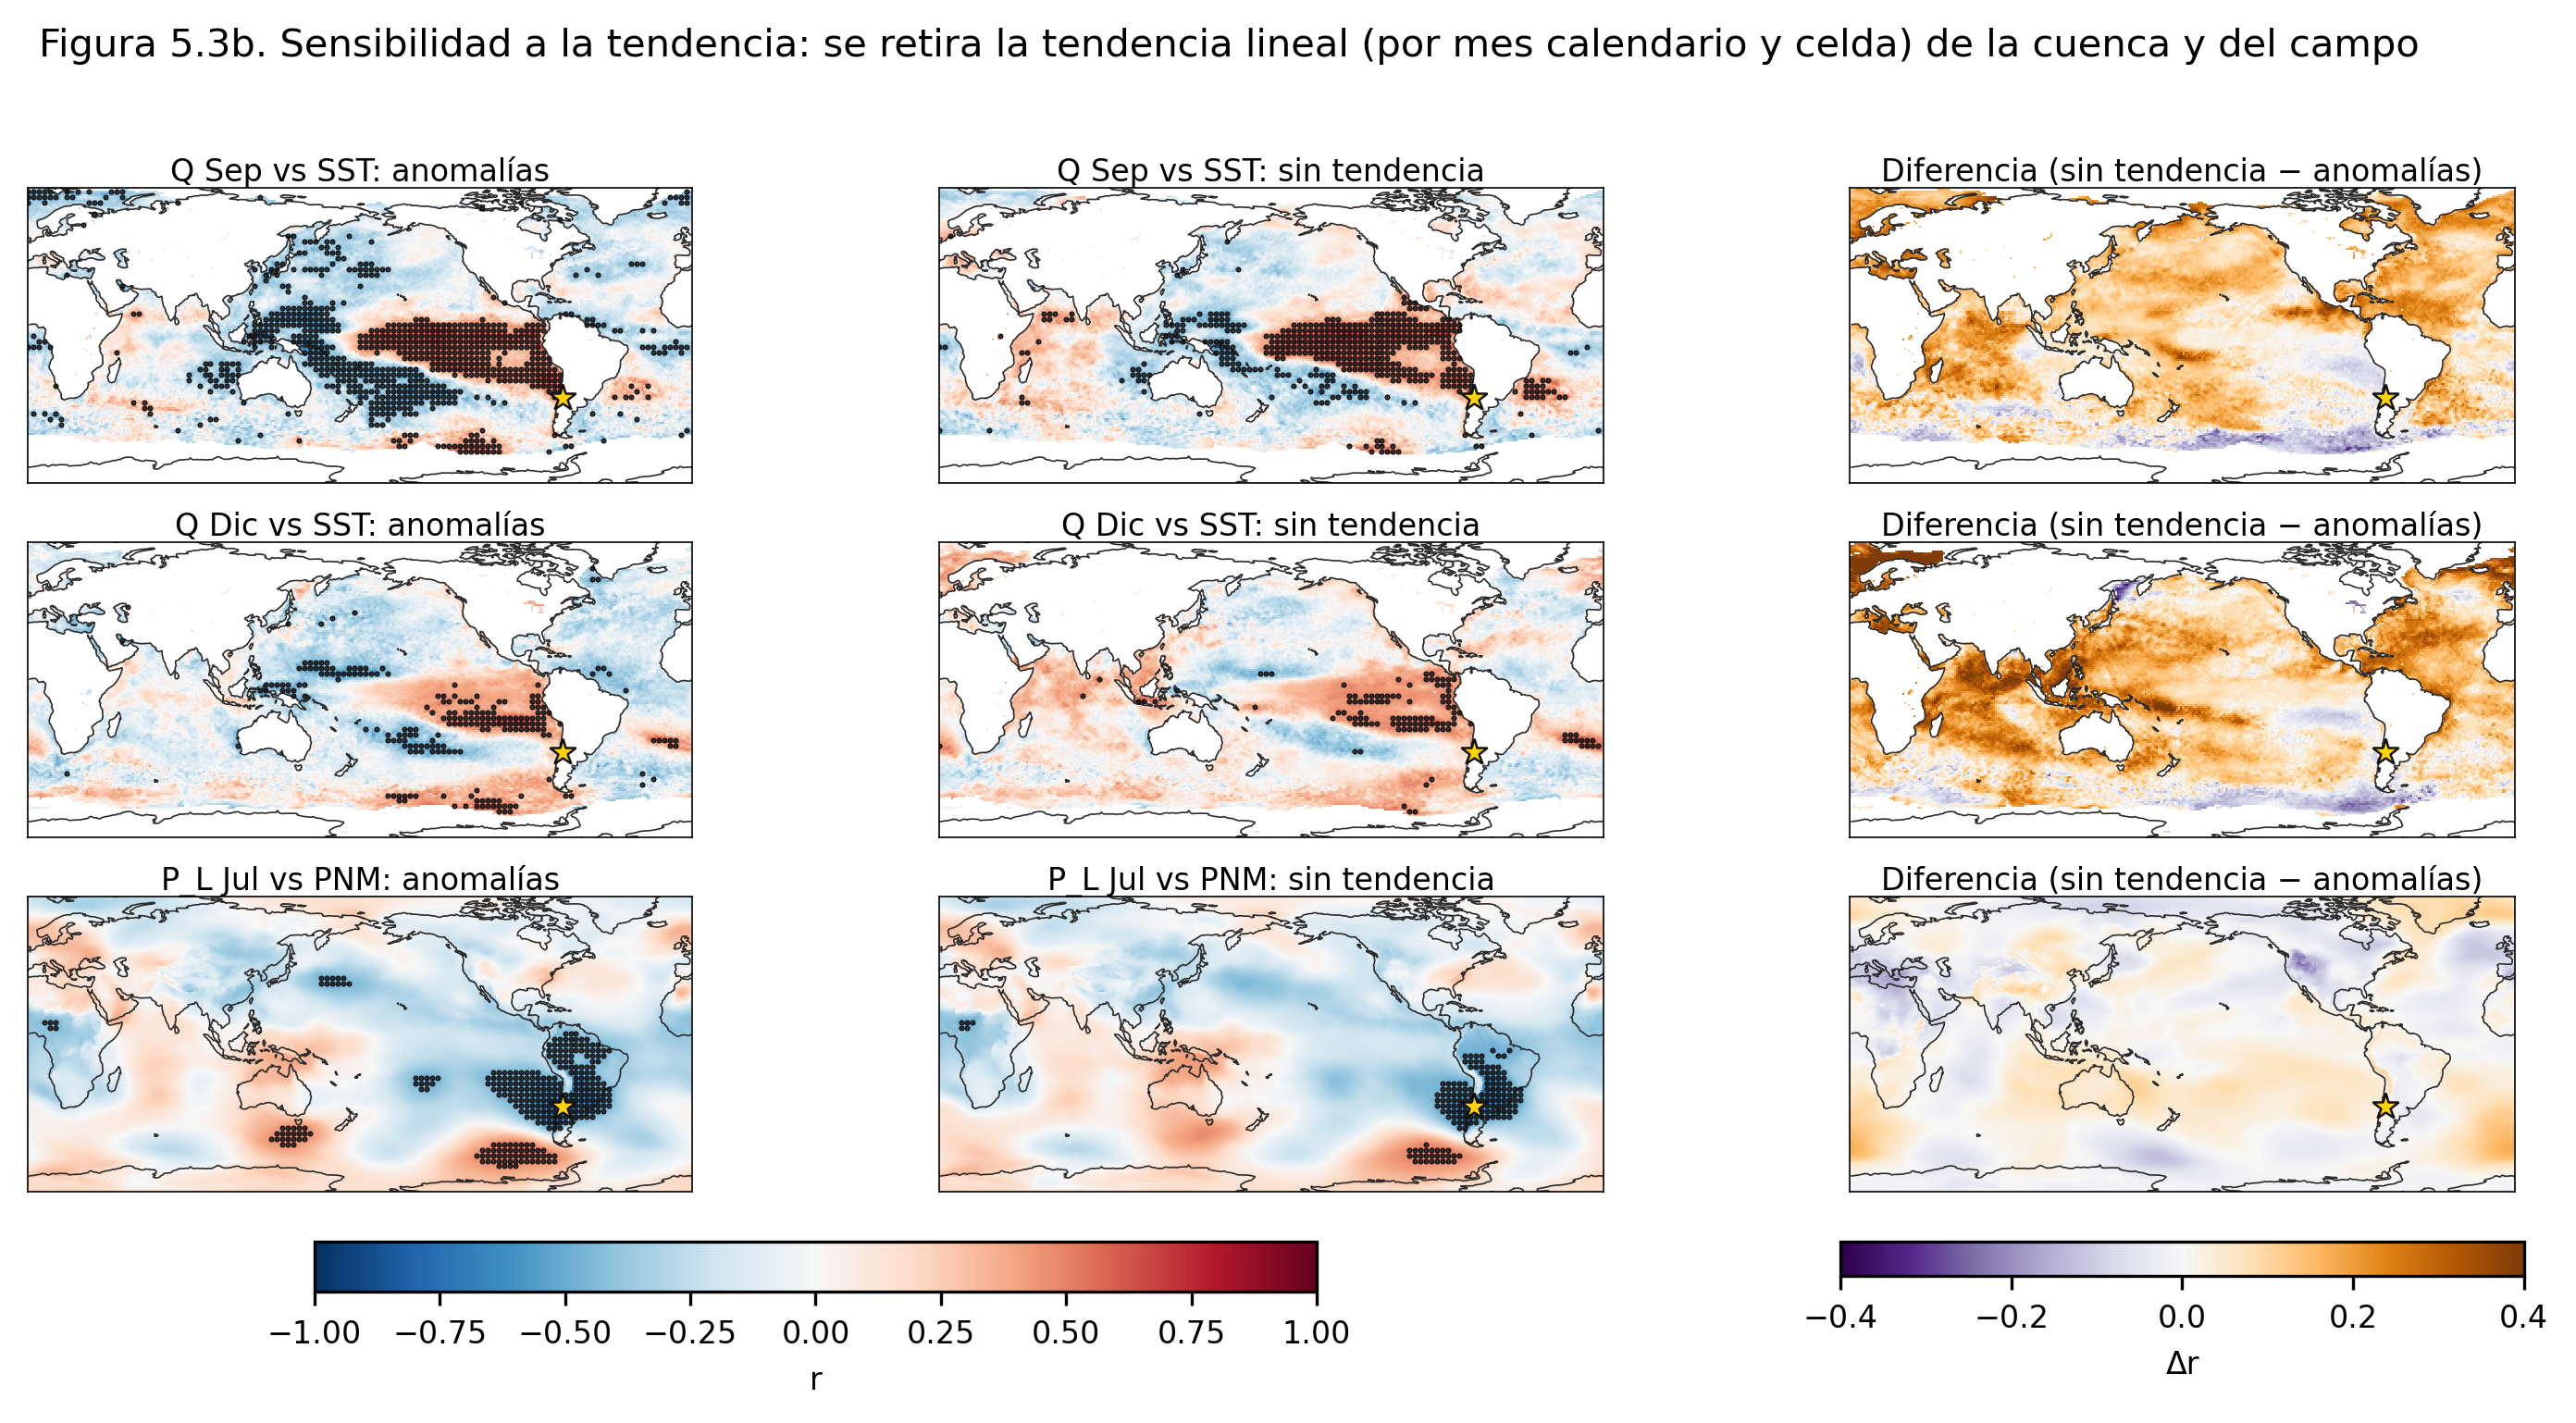
\includegraphics[width=\textwidth]{figura_5_3b_tendencia.png}
\caption{Correlación con anomalías, sin tendencia y diferencia, para $Q$ en septiembre y diciembre frente a la
SST y $P_L$ en julio frente a la PNM.}
\label{fig:tend}
\end{figure}

\paragraph{Estabilidad.} La Figura~\ref{fig:estab} resume tres pruebas, medidas con la correlación espacial de
patrones en el Pacífico (60$^\circ$S--60$^\circ$N, 120$^\circ$E--60$^\circ$W):
\begin{itemize}
\item \textbf{Años extremos}: retirar los 3 años de mayor anomalía de la cuenca en cada mes conserva los
patrones (mediana de 0.75--0.92).
\item \textbf{IMERG frente a $P_L$} con los mismos meses de 2000--2020: los patrones coinciden (mediana de
0.82--0.86), salvo en los meses secos de verano. La conclusión no depende de la fuente de precipitación en el
periodo común.
\item \textbf{Subperiodos} 1980--1999 frente a 2000--2019: a escala de toda la cuenca del Pacífico los
patrones \emph{no} se reproducen (mediana de 0.04--0.34). Con 20 años por mapa, el ruido muestral es grande, y
además hay no estacionariedad real (Sección~\ref{sec:interp}).
\end{itemize}

\begin{figure}[H]
\centering
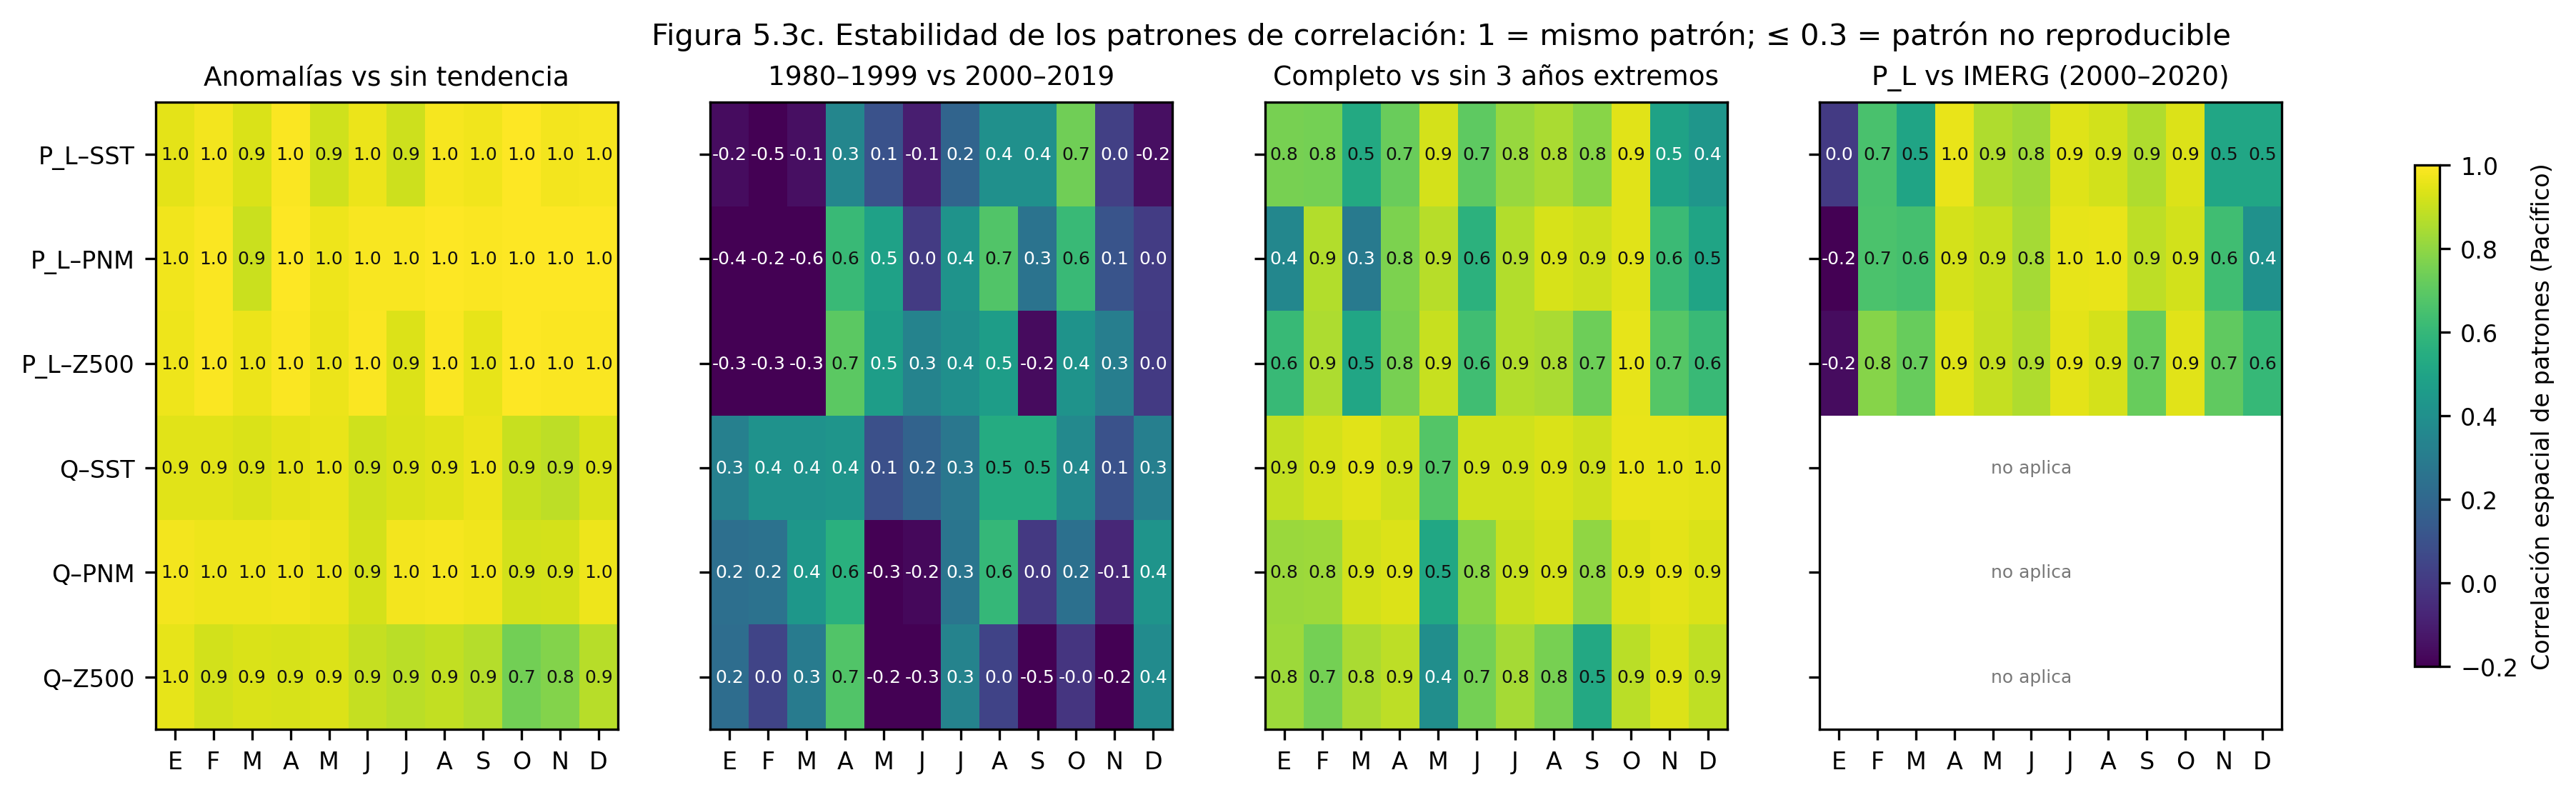
\includegraphics[width=\textwidth]{figura_5_3c_estabilidad.png}
\caption{Correlación espacial de patrones entre configuraciones, por combinación y mes.}
\label{fig:estab}
\end{figure}

\section{Interpretación física e integración (5.4)}
\label{sec:interp}

Para no elegir regiones a partir de los propios mapas, se definieron tres índices \emph{a priori} según el
mecanismo: Niño 3.4 (SST, 5$^\circ$S--5$^\circ$N, 170$^\circ$W--120$^\circ$W; \citealp{Trenberth1997}), la
PNM del Pacífico sureste (30--40$^\circ$S, 75--90$^\circ$W) y la Z500 sobre Chile central
(30--40$^\circ$S, 70--85$^\circ$W).

\begin{figure}[H]
\centering
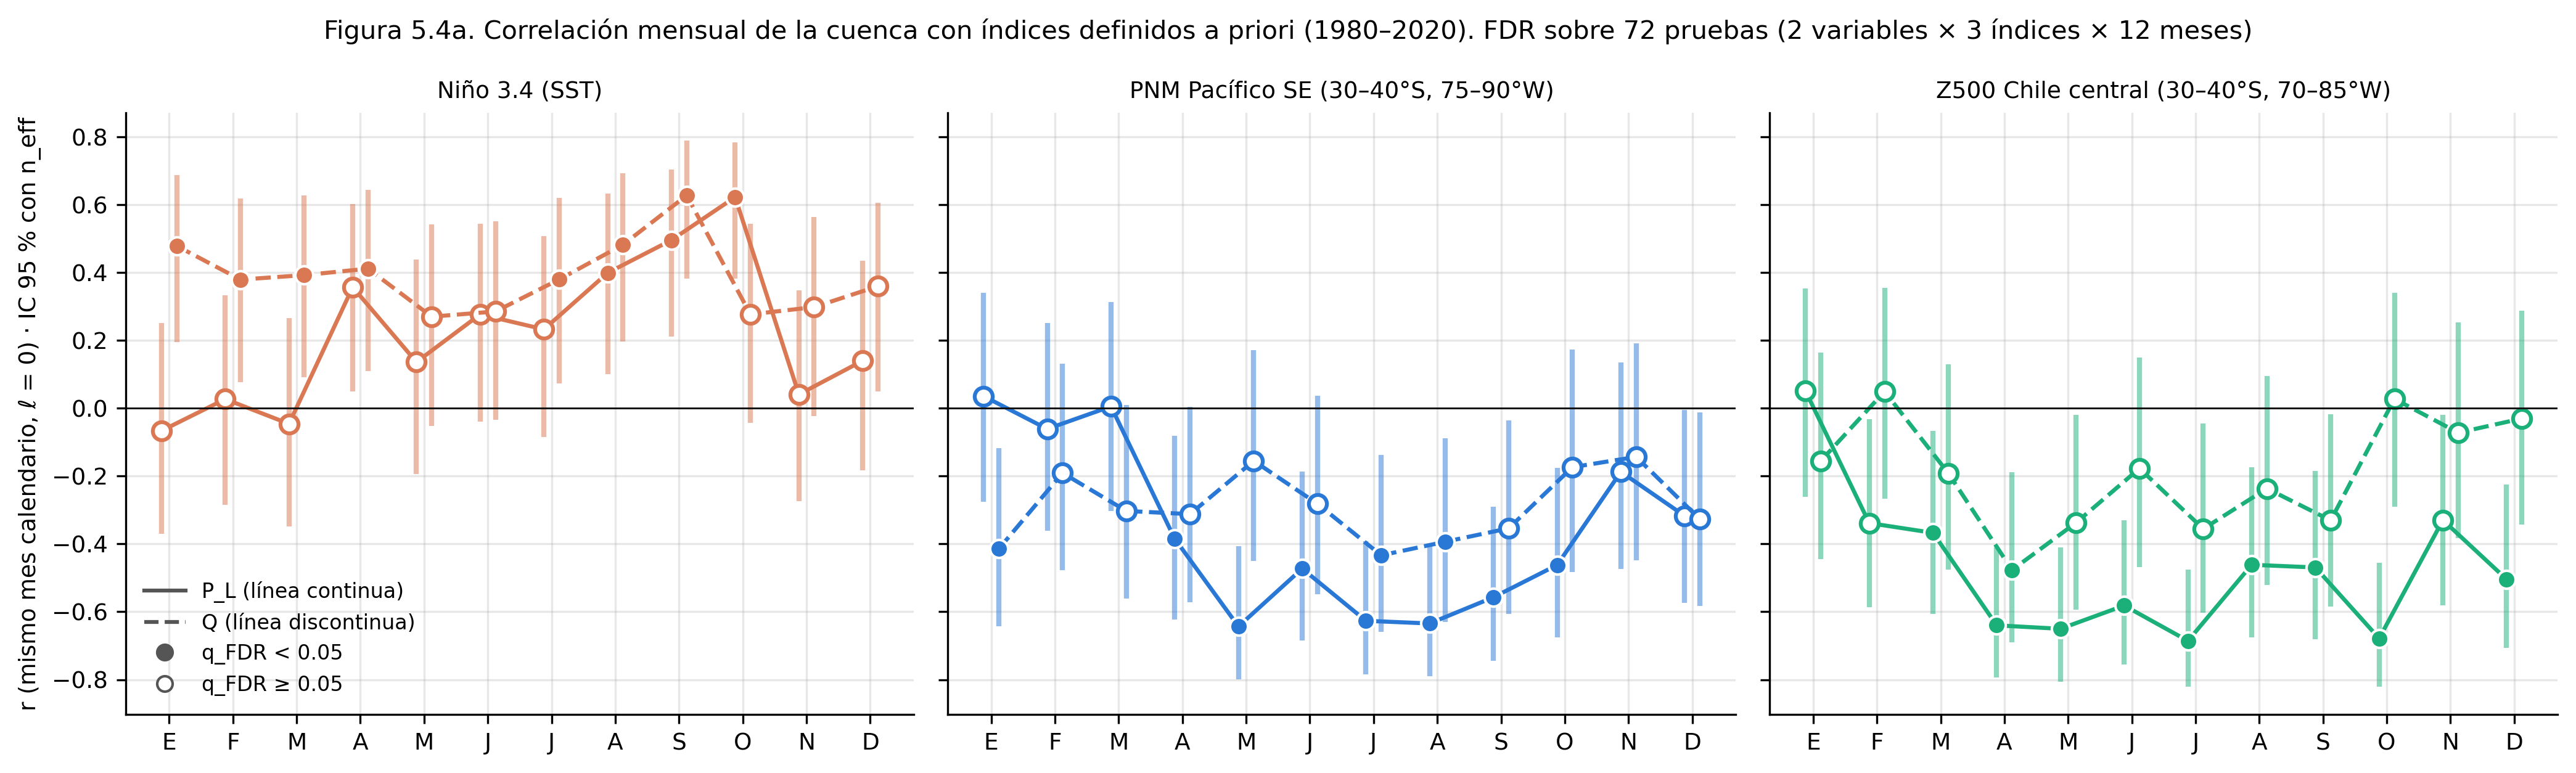
\includegraphics[width=\textwidth]{figura_5_4a_perfiles_indices.png}
\caption{Correlación mensual de $P_L$ (continua) y $Q$ (discontinua) con los tres índices; IC del 95\,\% con
$n_\mathrm{eff}$ y relleno si $q_\mathrm{FDR}<0.05$ (72 pruebas). Script \texttt{19\_p5\_4\_interpretacion.py}.}
\label{fig:perfiles}
\end{figure}

\paragraph{Regiones, signos y estaciones.} El resultado más sólido es \emph{local y atmosférico}. Entre abril y
octubre, $P_L$ se asocia con una PNM baja frente a Chile central ($r$ de $-0.38$ a $-0.64$) y con una Z500 baja
sobre la región ($r$ de $-0.46$ a $-0.69$); son 16 de las 30 pruebas significativas tras FDR
(Figura~\ref{fig:perfiles}). El mecanismo propuesto es que, cuando el anticiclón subtropical se debilita o se
desplaza al norte y una vaguada se instala frente a la costa, los sistemas frontales y las bajas segregadas
alcanzan los 33--34$^\circ$S y descargan lluvia orográfica sobre los Andes \citep{Garreaud2009}. El centro de
signo opuesto en las altas latitudes del Pacífico sur (Figura~\ref{fig:todos}) sugiere un patrón de tipo Modo
Anular del Sur: su fase positiva desplaza los oestes al sur y seca Chile central \citep{Gillett2006}. Esta
hipótesis es compatible con nuestros mapas, pero no se probó con un índice SAM. La asociación con la SST
tropical es \emph{más débil y tardía}: $P_L$ con Niño 3.4 solo es significativa en agosto--octubre ($r=0.40$,
0.50 y 0.62). Eso concuerda con la estacionalidad documentada de la señal de ENSO en Chile central, más fuerte
hacia fines del invierno y en primavera \citep{Montecinos2003}.

\paragraph{¿Los patrones atmosféricos apoyan la explicación de la SST?} Parcialmente, y los campos no son
independientes. Niño 3.4 y la PNM local covarían ($r$ de $-0.28$ a $-0.49$ entre julio y diciembre). Al
controlar por la PNM, la correlación parcial de $P_L$ con Niño 3.4 baja (julio: de 0.23 a 0.06; agosto: de 0.40
a 0.20; octubre: de 0.62 a 0.52), mientras que la de $P_L$ con la PNM casi no cambia al controlar por Niño 3.4
(julio: de $-0.63$ a $-0.60$). La lectura es que ENSO actúa en buena parte \emph{a través} de la circulación
local (El Niño debilita el anticiclón y favorece bloqueos en el Pacífico sureste;
\citealp{Rutllant1991,Montecinos2003}), pero esa circulación también varía por causas no relacionadas con ENSO.
Las correlaciones separadas no son influencias independientes.

\paragraph{¿Coinciden los meses de mayor asociación para $P$ y $Q$? ¿El rezago es compatible?} No coinciden, y
esa diferencia es informativa. $Q$ se asocia positivamente con Niño 3.4 \emph{todo el año} (0.27--0.63; 7 meses
significativos tras FDR), incluido el verano, cuando casi no llueve. La Figura~\ref{fig:rezagos} explica por qué:
el caudal de octubre a marzo correlaciona fuertemente con la lluvia de mayo--agosto previa ($r=0.84$--0.92) y,
de forma más débil, con Niño 3.4 de ese invierno ($r=0.32$--0.42). Esto respalda la cadena
\emph{ENSO $\rightarrow$ lluvia invernal $\rightarrow$ nieve $\rightarrow$ caudal de deshielo}: el almacenamiento
nival traslada la señal de invierno al verano, y la persistencia de ENSO durante varios meses la extiende
(la matriz de rezagos muestra $r\approx0.5$ entre el caudal de abril y Niño 3.4 de 1 a 8 meses antes). El
rezago de 6 meses es físicamente coherente, pero no domina sobre la correlación contemporánea, porque Niño 3.4
persiste. Es una asociación simultánea y no se evaluó su capacidad de pronóstico fuera de muestra.

\begin{figure}[H]
\centering
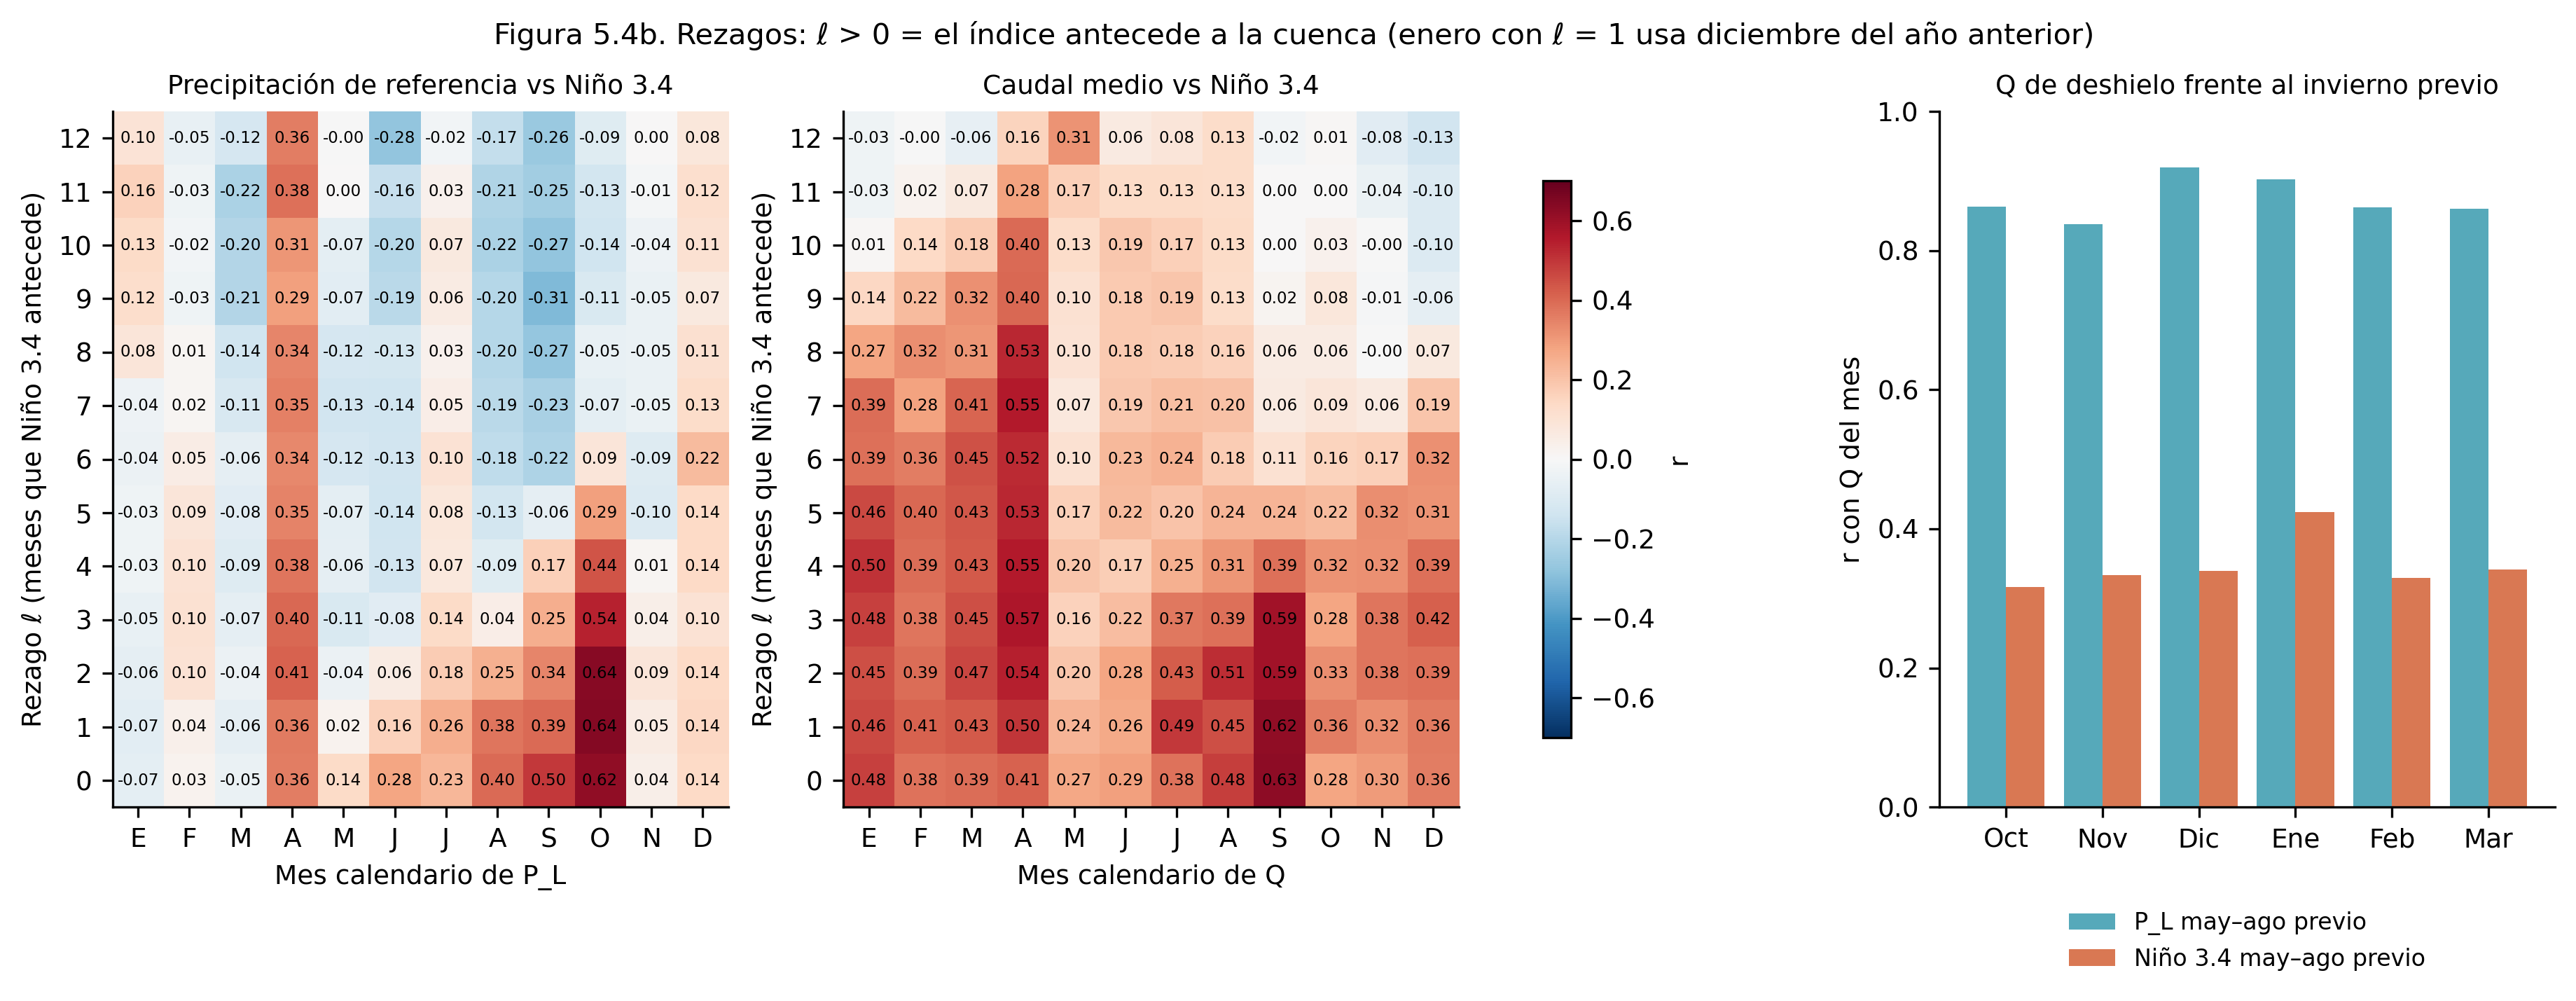
\includegraphics[width=\textwidth]{figura_5_4b_rezagos_nino34.png}
\caption{Correlación de $P_L$ y $Q$ con Niño 3.4 por mes y rezago, y caudal de deshielo frente a la lluvia y
a Niño 3.4 del invierno previo.}
\label{fig:rezagos}
\end{figure}

\paragraph{No estacionariedad.} La relación entre la PNM local y $P_L$ es estable en pleno invierno
(mayo--agosto: de $-0.41$ a $-0.74$ en 1980--1999 y de $-0.49$ a $-0.59$ en 2000--2019), pero se debilita en
septiembre--octubre. La relación entre $Q$ y Niño 3.4 \emph{cae} fuertemente después de 2000 (septiembre: 0.81
frente a 0.31; enero: 0.74 frente a 0.14; Figura~\ref{fig:sub}). La explicación alternativa más plausible es la
megasequía: entre 2010 y 2019 la lluvia y el caudal fueron bajos con independencia de la fase de ENSO, y el
Niño intenso de 2015 no trajo la lluvia esperada \citep{Garreaud2017,Garreaud2020}. Esto sugiere que un control
de baja frecuencia (Pacífico extratropical, tendencia del Modo Anular del Sur) se superpuso a ENSO. Con 20 años
por subperiodo no se puede separar ese cambio real del ruido muestral.

\begin{figure}[H]
\centering
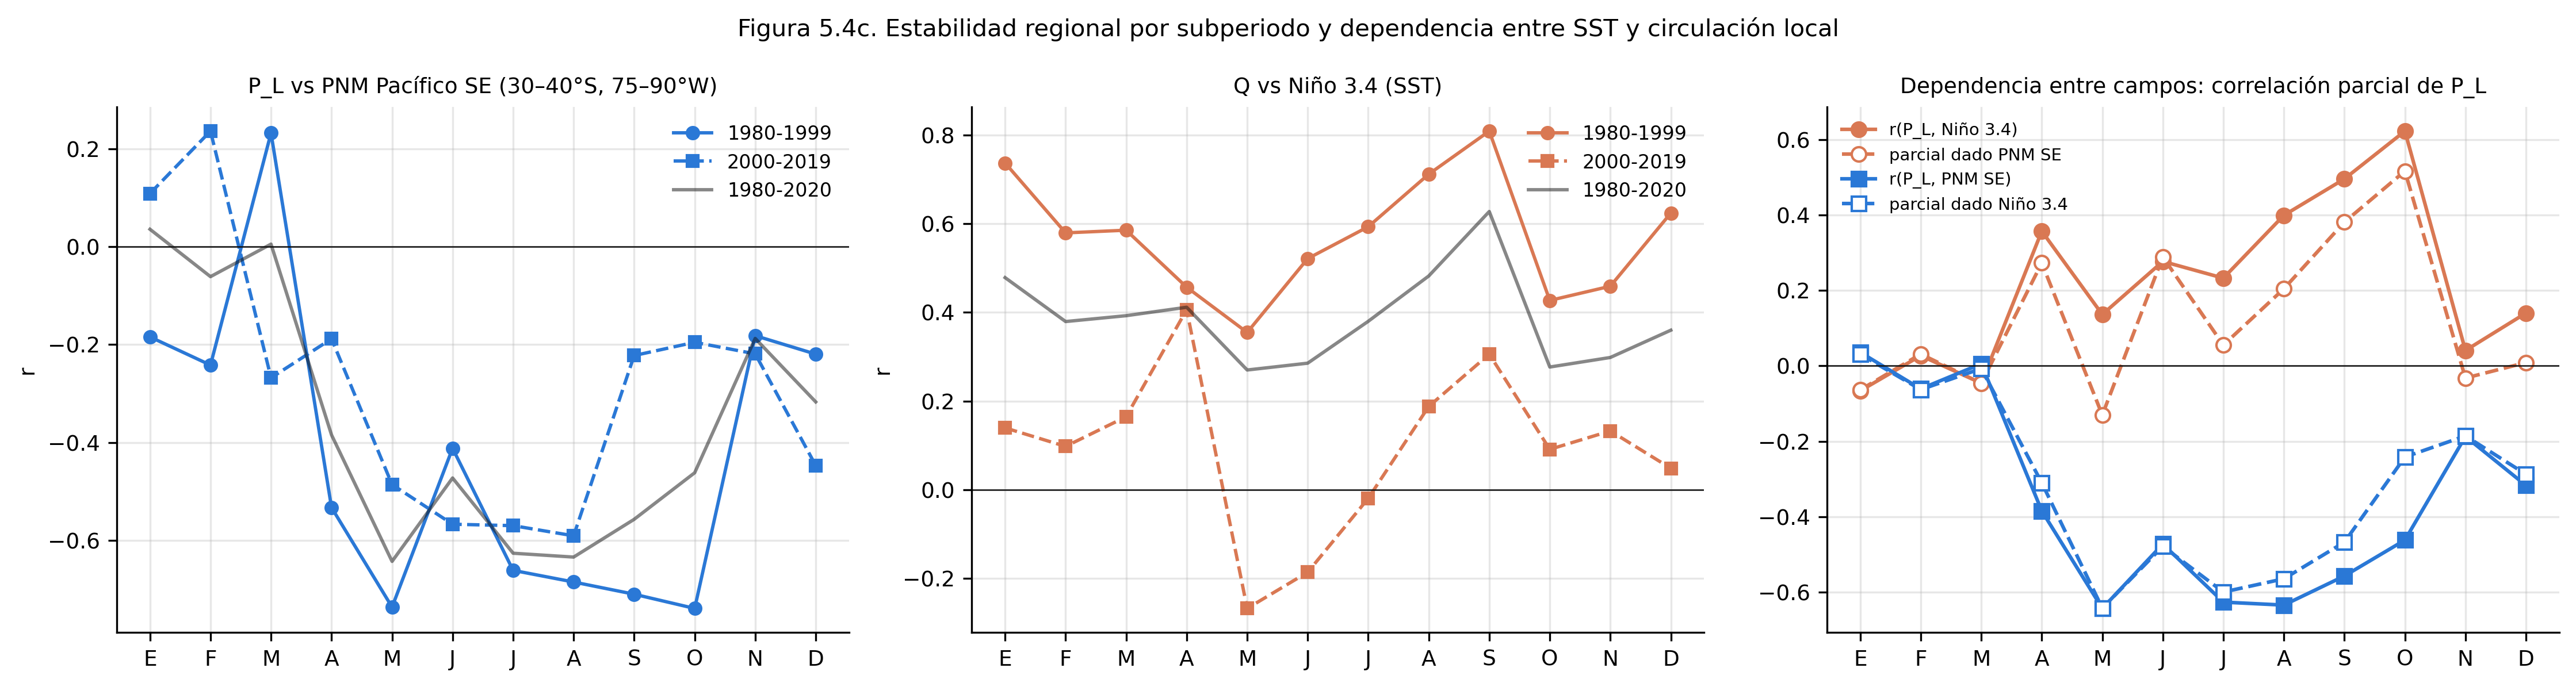
\includegraphics[width=\textwidth]{figura_5_4c_subperiodos_parcial.png}
\caption{Correlación por subperiodo ($P_L$--PNM y $Q$--Niño 3.4) y correlación parcial de $P_L$ con Niño 3.4 y
con la PNM local.}
\label{fig:sub}
\end{figure}

\paragraph{Relación con las bandas del punto 4.} El punto 4 no encontró un pico interanual robusto: la
varianza interanual del caudal es una banda ancha de ruido rojo. Coherentemente, la coherencia espectral entre
las anomalías de la cuenca y Niño 3.4 es moderada (Figura~\ref{fig:coh}): media de 0.30 ($P_L$) y 0.27 ($Q$) en
la banda de 2--7 años, con máximos de 0.46--0.49 cerca de 5 años que apenas superan el umbral aproximado del
95\,\% (0.39). Compartir la banda de ENSO no demuestra por sí solo una conexión causal. Lo que la sustenta es
la combinación de un mecanismo conocido, los patrones espaciales coherentes y la cadena de rezagos.

\begin{figure}[H]
\centering
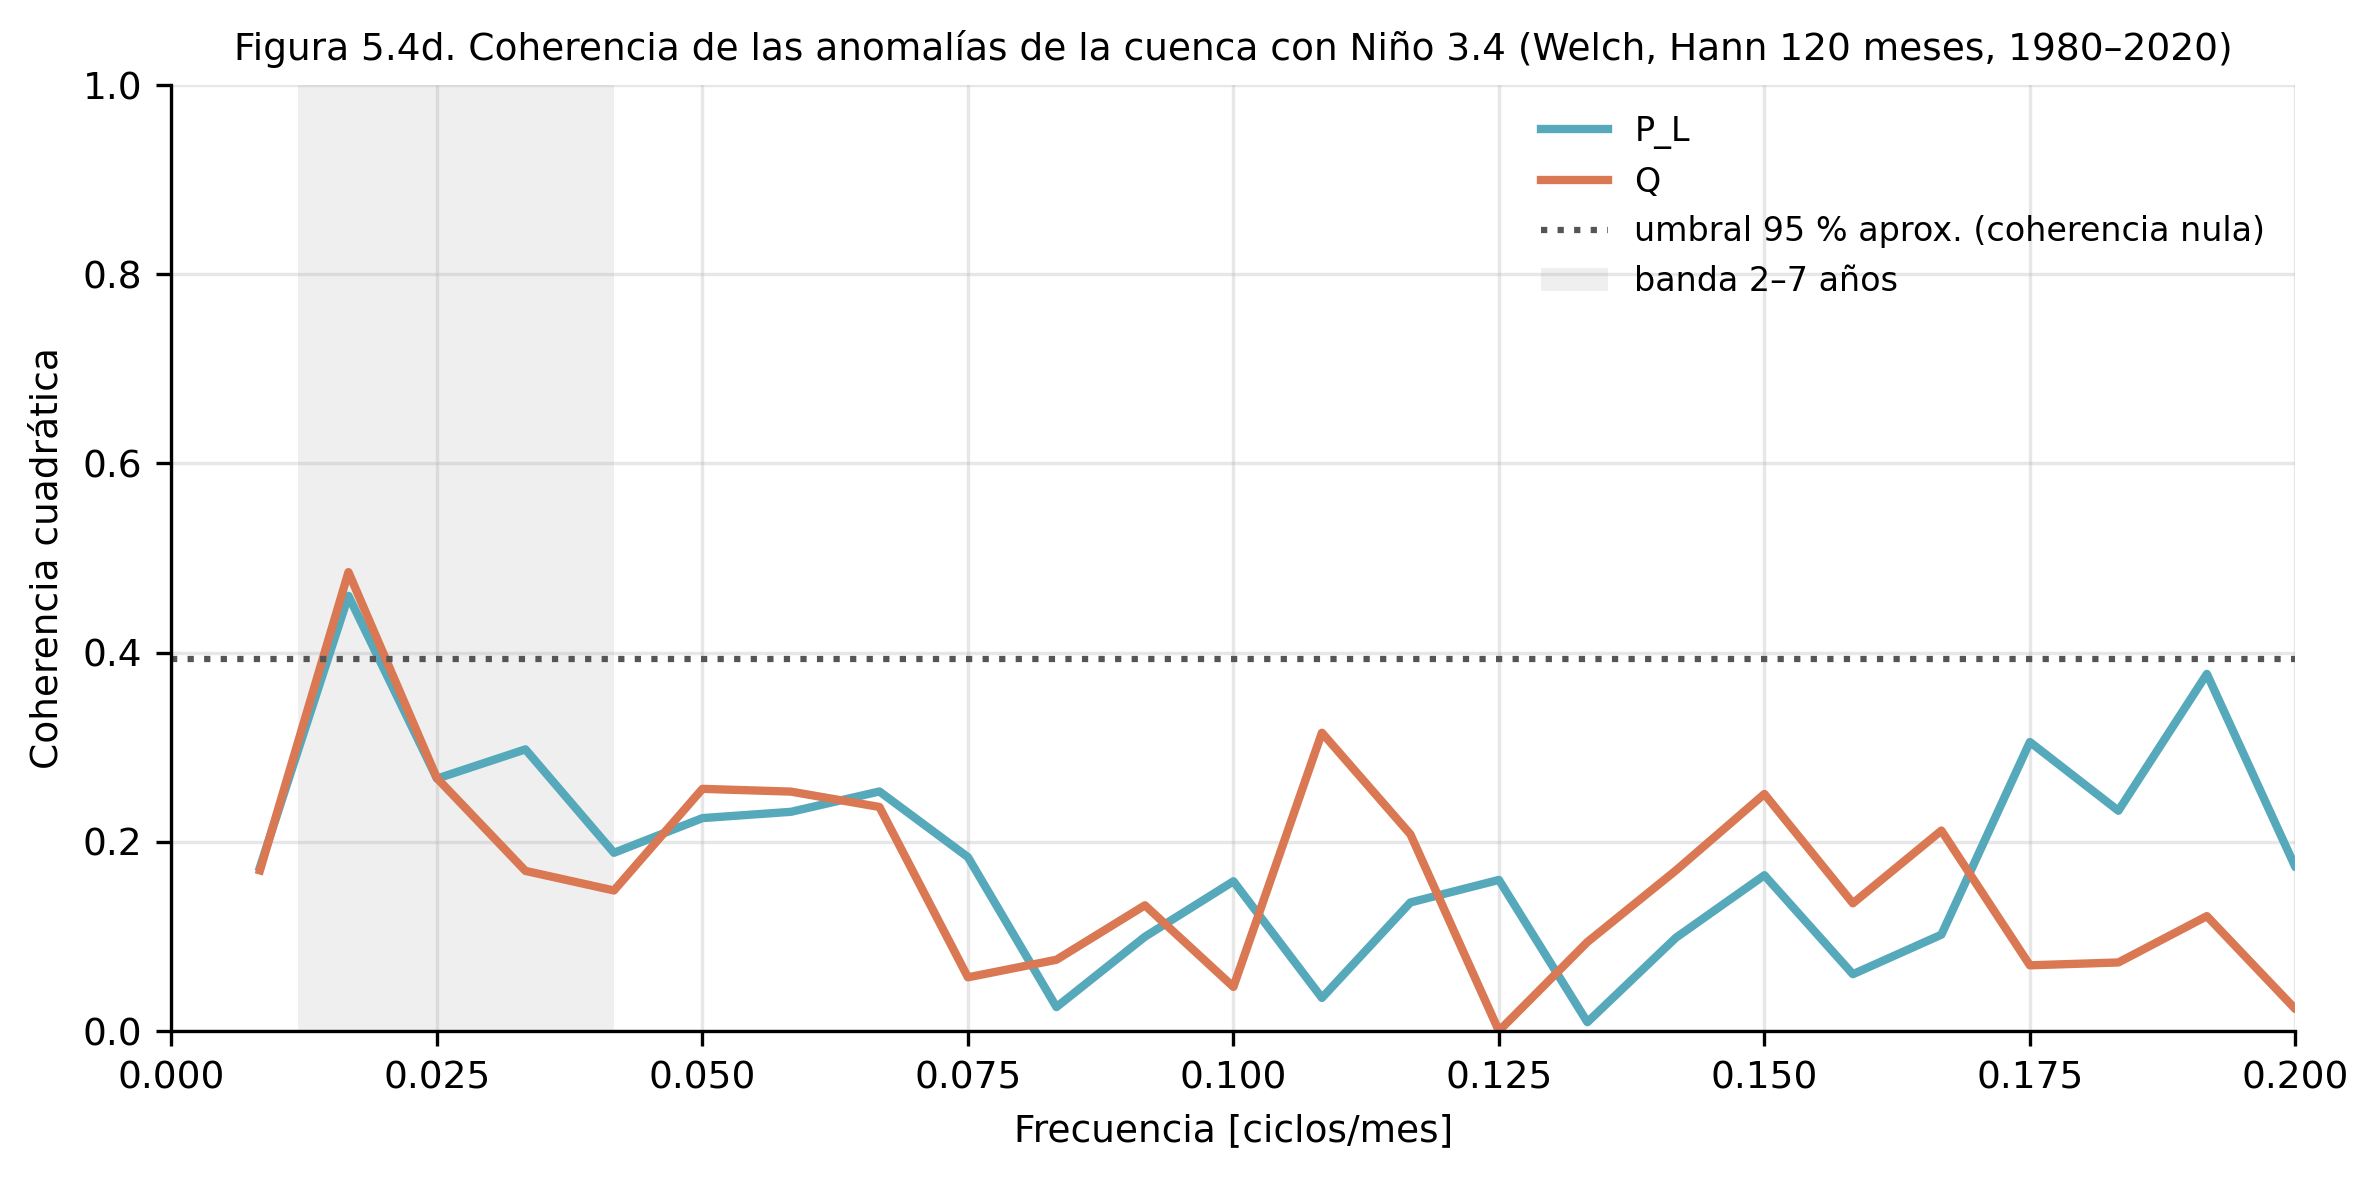
\includegraphics[width=0.75\textwidth]{figura_5_4d_coherencia.png}
\caption{Coherencia cuadrática entre las anomalías de $P_L$ o $Q$ y Niño 3.4 (Welch, Hann de 120 meses,
1980--2020).}
\label{fig:coh}
\end{figure}

\begin{tcolorbox}[colback=blue!3,colframe=blue!50!black,title=Síntesis de los puntos 4 y 5,fonttitle=\bfseries]
\textbf{Resultados sólidos.} (1) La escala dominante es el ciclo anual (punto 4); la variabilidad interanual del
caudal es una banda ancha y roja, filtrada por el almacenamiento nival. (2) La lluvia de abril a octubre se
asocia con una circulación local de baja presión y vaguada frente a Chile central (PNM y Z500; $|r|\approx0.5$--0.7,
significativa tras FDR y estable en pleno invierno en ambos subperiodos).

\textbf{Asociaciones exploratorias.} (3) La SST tropical (ENSO) se asocia con la lluvia de agosto a octubre y con
el caudal de todo el año, transmitida por la nieve; actúa en parte a través de la circulación local y se
debilitó después de 2000. (4) Un dipolo en la PNM de altas latitudes, compatible con el Modo Anular del Sur.

\textbf{No comprobado.} El papel causal del Modo Anular del Sur o del Pacífico extratropical en la megasequía,
y cualquier capacidad de pronóstico. No hubo patrones claros con la Z500 para el caudal ni con la SST para la
lluvia de verano.
\end{tcolorbox}

\begin{thebibliography}{99}\small
% VERIFICAR: comprobar cada referencia (autores, año, páginas y DOI) contra la fuente original.
\bibitem{BH1995} Benjamini, Y., y Hochberg, Y. (1995). Controlling the false discovery rate: a practical and powerful approach to multiple testing. \emph{Journal of the Royal Statistical Society B}, 57, 289--300. \url{https://doi.org/10.1111/j.2517-6161.1995.tb02031.x}
\bibitem{Bretherton1999} Bretherton, C. S., Widmann, M., Dymnikov, V. P., Wallace, J. M., y Bladé, I. (1999). The effective number of spatial degrees of freedom of a time-varying field. \emph{Journal of Climate}, 12, 1990--2009. \url{https://doi.org/10.1175/1520-0442(1999)012<1990:TENOSD>2.0.CO;2}
\bibitem{Garreaud2009} Garreaud, R. D., Vuille, M., Compagnucci, R., y Marengo, J. (2009). Present-day South American climate. \emph{Palaeogeography, Palaeoclimatology, Palaeoecology}, 281, 180--195. \url{https://doi.org/10.1016/j.palaeo.2007.10.032}
\bibitem{Garreaud2017} Garreaud, R. D., Alvarez-Garreton, C., Barichivich, J., et al. (2017). The 2010--2015 megadrought in central Chile: impacts on regional hydroclimate and vegetation. \emph{Hydrology and Earth System Sciences}, 21, 6307--6327. \url{https://doi.org/10.5194/hess-21-6307-2017}
\bibitem{Garreaud2020} Garreaud, R. D., Boisier, J. P., Rondanelli, R., et al. (2020). The Central Chile Mega Drought (2010--2018): A climate dynamics perspective. \emph{International Journal of Climatology}, 40, 421--439. \url{https://doi.org/10.1002/joc.6219}
\bibitem{Gillett2006} Gillett, N. P., Kell, T. D., y Jones, P. D. (2006). Regional climate impacts of the Southern Annular Mode. \emph{Geophysical Research Letters}, 33, L23704. \url{https://doi.org/10.1029/2006GL027721}
\bibitem{Hersbach2020} Hersbach, H., Bell, B., Berrisford, P., et al. (2020). The ERA5 global reanalysis. \emph{Quarterly Journal of the Royal Meteorological Society}, 146, 1999--2049. \url{https://doi.org/10.1002/qj.3803}
\bibitem{Montecinos2003} Montecinos, A., y Aceituno, P. (2003). Seasonality of the ENSO-related rainfall variability in central Chile and associated circulation anomalies. \emph{Journal of Climate}, 16, 281--296. \url{https://doi.org/10.1175/1520-0442(2003)016<0281:SOTERR>2.0.CO;2}
\bibitem{Rutllant1991} Rutllant, J., y Fuenzalida, H. (1991). Synoptic aspects of the central Chile rainfall variability associated with the Southern Oscillation. \emph{International Journal of Climatology}, 11, 63--76. \url{https://doi.org/10.1002/joc.3370110105}
\bibitem{Trenberth1997} Trenberth, K. E. (1997). The definition of El Niño. \emph{Bulletin of the American Meteorological Society}, 78, 2771--2777. \url{https://doi.org/10.1175/1520-0477(1997)078<2771:TDOENO>2.0.CO;2}
\bibitem{Wilks2016} Wilks, D. S. (2016). ``The stippling shows statistically significant grid points'': How research results are routinely overstated and overinterpreted, and what to do about it. \emph{Bulletin of the American Meteorological Society}, 97, 2263--2273. \url{https://doi.org/10.1175/BAMS-D-15-00267.1}
\end{thebibliography}

\end{document}
